\chapter{Implementation and Tests}

\section{Introduction}

After completing the design of our solution in the previous chapter, this chapter focuses on its concrete implementation and testing. We detail the development process of the system components, including the integration of the deep learning models for both wheat disease classification and insect pest detection.

We also explain how these models were deployed into a functional and accessible web platform tailored for farmers. The implementation of the AI assistant is also covered, highlighting how it supports users through an interactive and user-friendly interface. Finally, this chapter presents the different tests conducted to verify the behavior, functionality, and robustness of the system in real conditions. These tests help ensure that the system performs as intended and is ready for practical deployment.



\section{Development Environment}
Training the proposed wheat-health models required the use of two distinct compute setups. For the wheat-disease classification task, we initially relied on Google Colab’s free cloud instances due to the absence of a local \gls{abb:gpu}, conducting all training and experimentation in the cloud. Later, for the insect-pest detection task and integration efforts, we utilized a laptop equipped with an NVIDIA RTX 4050 \gls{abb:gpu}, which enabled faster processing and reproducible experiments to be executed locally. More details on the hardware specifications are provided in Table~\ref{tab:hardware-specs}.

\begin{table}[H]
    \caption{Hardware specifications by task}
    \centering
    \resizebox{\textwidth}{!}{%
    \begin{tabular}{|p{4.2cm}|p{5.5cm}|p{5.5cm}|}
        \hline
        \textbf{Component} & \textbf{Wheat-Disease Classification (Google Colab)} & \textbf{Insect-Pest Detection (Local Laptop)} \\
        \hline
        Processor & Intel Xeon or equivalent (shared cloud CPU) & AMD Ryzen 5  \\
        \hline
        GPU & T4 GPU (allocated per session) & NVIDIA GeForce RTX 4050  \\
        \hline
        System Memory & 12 GB & 16 GB  \\
        \hline
        Storage & Limited Google Drive storage & 475 GB SSD \\
        \hline
    \end{tabular}%
    }
    \label{tab:hardware-specs}
\end{table}

A consistent and modular software toolchain was used to support all stages of development, from data preparation to model training and deployment. Full details on the tools, libraries, and configurations are provided in Appendix \ref{app:annexC}.



\section{Implementation of the AI Assistant}

This AI assistant is powered by Google's Gemini API and allows users to input questions or photos of wheat crops to receive real-time AI-generated feedback.The assistant was implemented as a web API using the Flask microframework.The entire process from user input to response generation and return is visually summarized in Figure~\ref{fig:chatbot-process}. The main components are described below:

\begin{itemize}
    \item \textbf{API access key acquisition:}  
    An API key was obtained from the Google AI Studio platform, which grants access to the Gemini models via the \texttt{google.generativeai} Python package.

    \item \textbf{Environment variable configuration:}  
    To secure the API key and prevent hardcoding, it was stored in an \texttt{.env} file. This variable is loaded securely during runtime to configure the Gemini SDK.

    \item \textbf{Setting up Flask with CORS:}  
    A Flask server was initialized to handle HTTP requests. CORS (Cross-Origin Resource Sharing) was enabled to allow access from front-end applications hosted on different domains.

    \item \textbf{Gemini Flash model integration:}  
    The \texttt{gemini-1.5-flash} model was selected due to its efficiency and support for both image and text inputs. The model was initialized once using the configured API key.

    \item \textbf{Handling chat requests:}  
    The endpoint \texttt{/chatbot} listens for POST requests containing either a textual message, an image, or both. Submitted images are validated for allowed file types and verified to ensure they are readable.

    \item \textbf{Sending requests to Gemini:}  
    If the input is valid, the message and/or image are appended to a content list and sent to the Gemini model using the \texttt{generate\_content} method. The response is then extracted and returned to the front end in JSON format.

    \item \textbf{Error handling:}  
    Proper exception handling is implemented to catch unexpected runtime issues and return appropriate error messages to the client, while logging them on the server.
\end{itemize}



\begin{figure}[H]
\centering
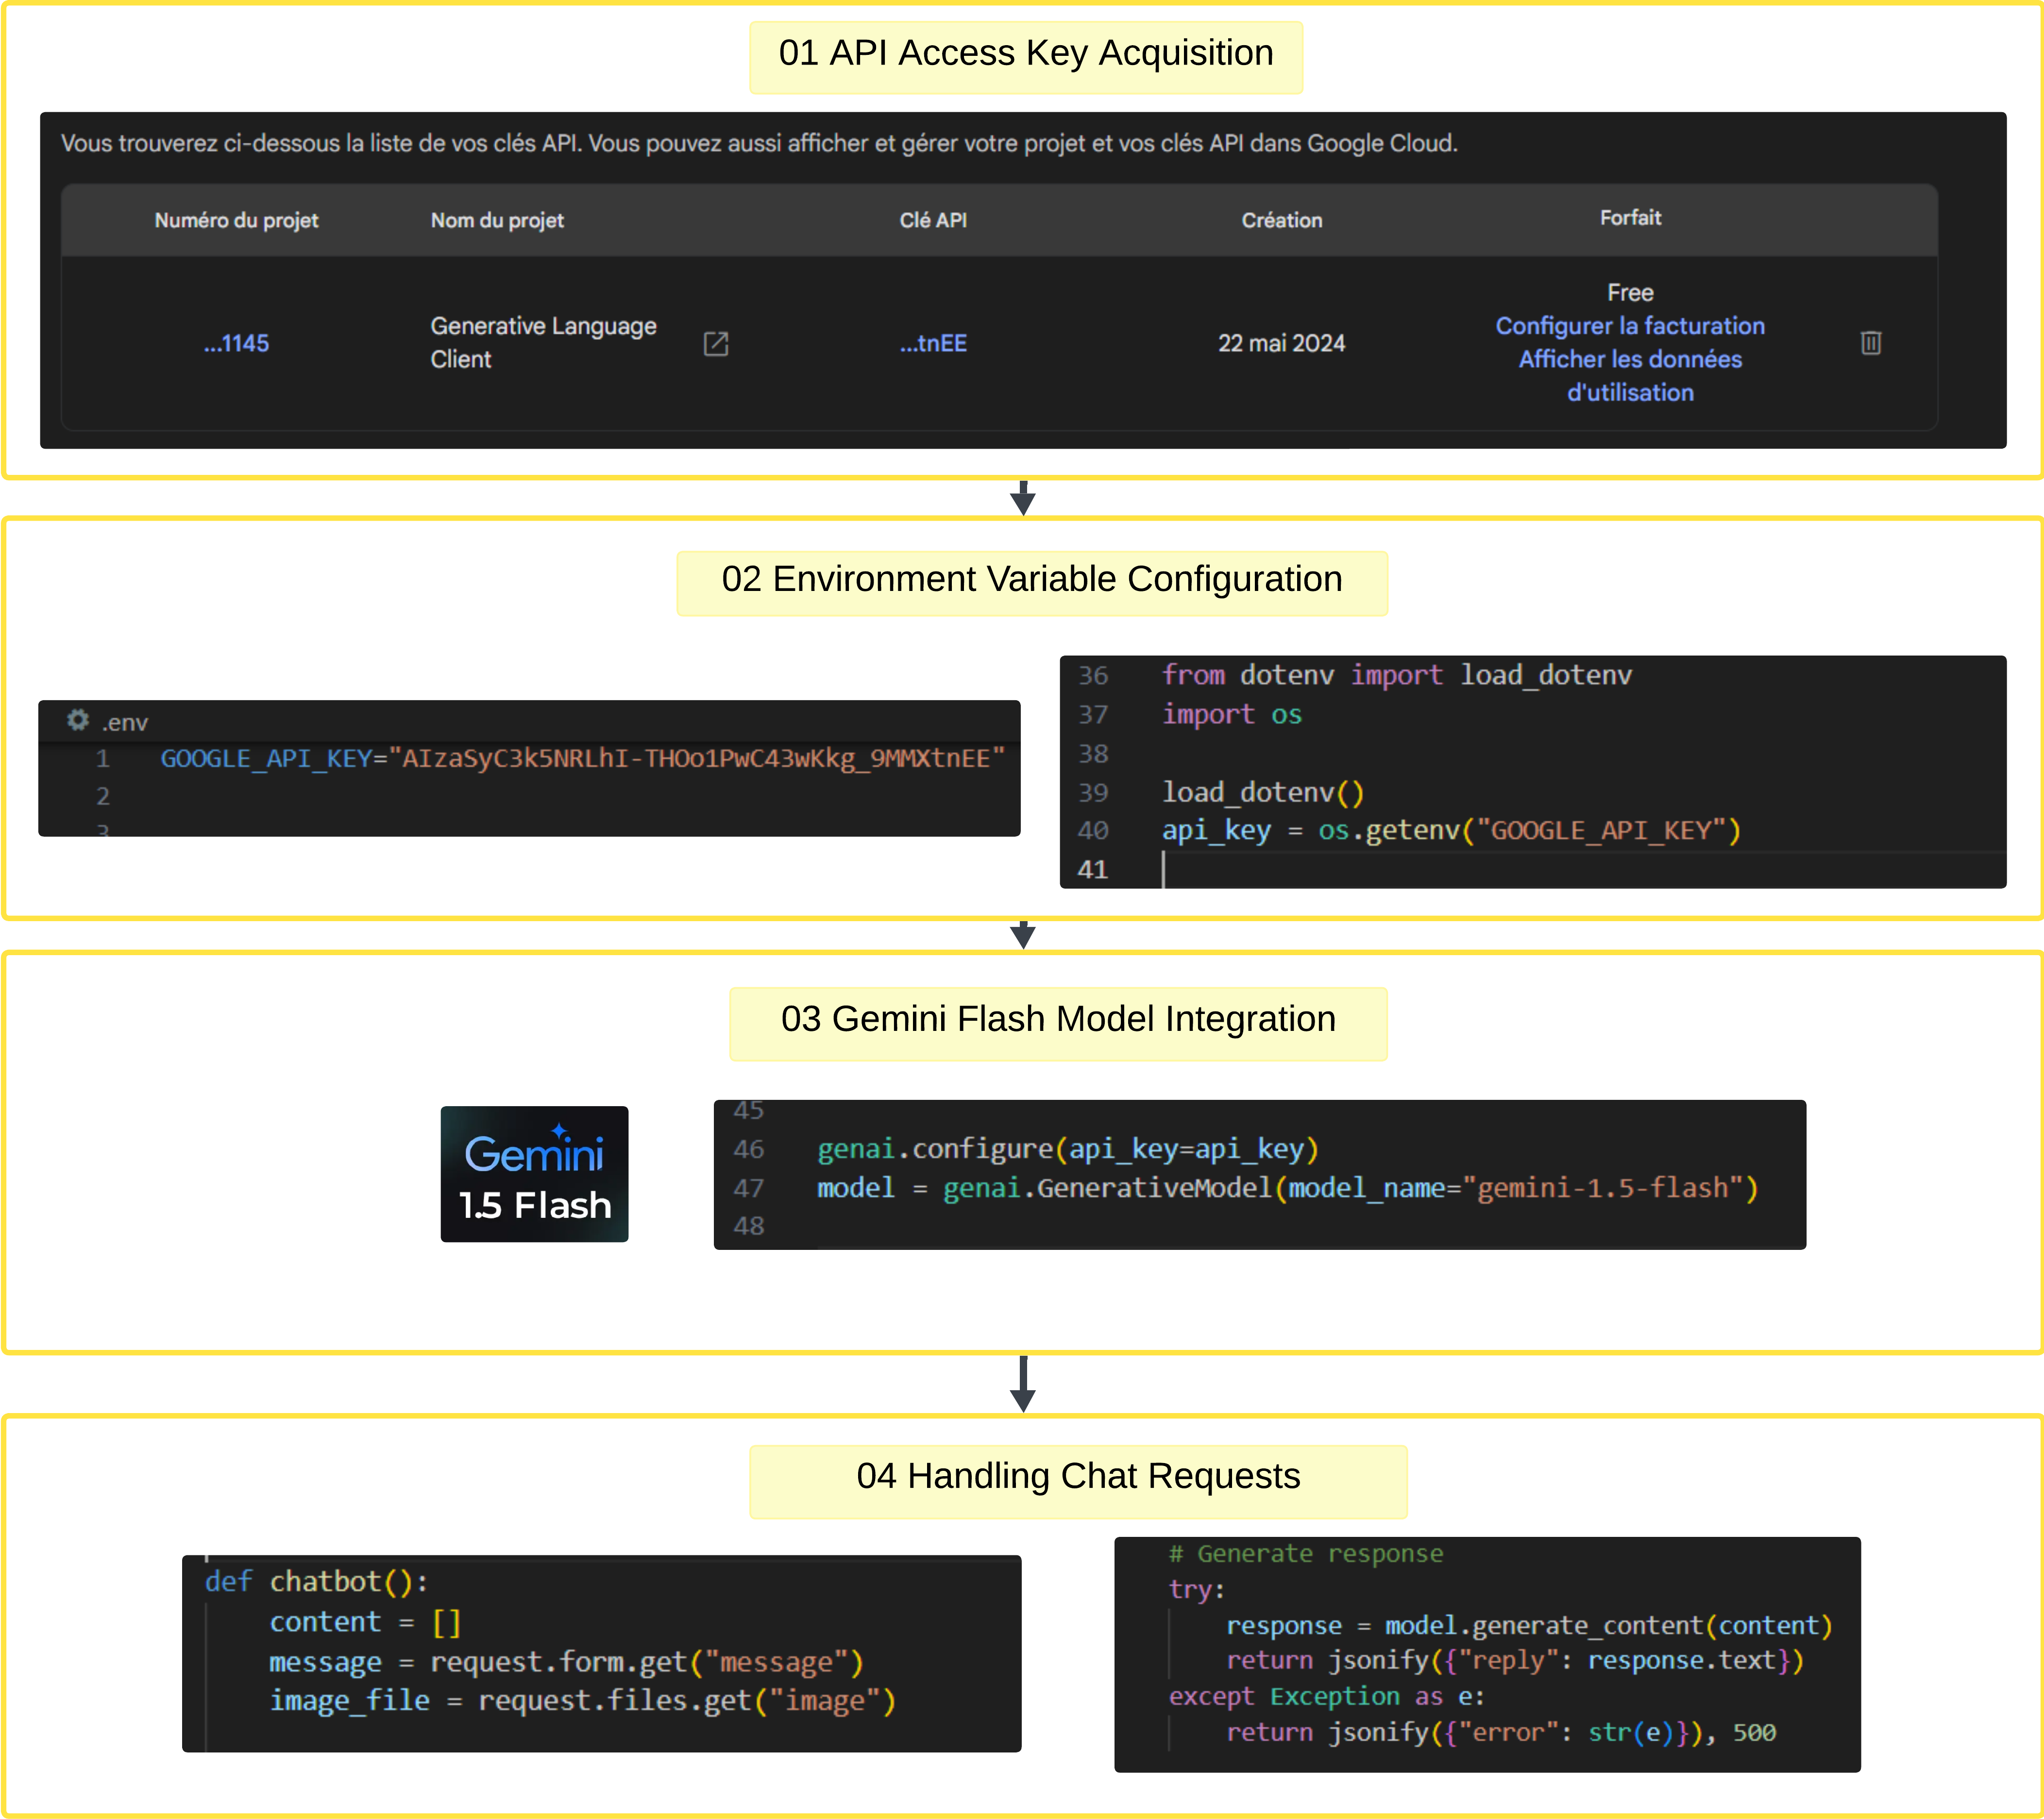
\includegraphics[width=1\textwidth]{chapters/chapter56/images/Figure13.png}
\caption{Pipeline of the AI assistant from input reception to Gemini-based response generation.}
\label{fig:chatbot-process}
\end{figure}



\section{Implementation of the web platform}
The deployment of the trained models was carried out through the Wheat Guard web platform, enabling real-time interaction with users. The platform also features intuitive interfaces that support image uploads, disease classification, and pest detection functionalities.
\subsection{Model integration}
In machine learning and deep learning workflows, saving trained models is a key step, whether for future inference, continued fine-tuning, or deployment. The choice of file format depends on the framework used and the intended purpose. Gaining a solid understanding of these formats ensures efficient model management and smooth transitions throughout the development pipeline.

\begin{itemize}
    \item \textbf{.pkl}: Commonly used with traditional machine learning libraries like \texttt{scikit-learn}, this format stores complete Python objects, including trained models, using Python’s \texttt{Pickle} serialization protocol.

    \item \textbf{.pth / .pt}: These formats are native to \texttt{PyTorch}. They are used to save model weights or full models. While functionally similar, \texttt{.pt} is generally preferred for deployment, especially when models are exported with \texttt{TorchScript}.

    \item \textbf{.h5}: Used by \texttt{Keras} and \texttt{TensorFlow}, this format (based on the \texttt{HDF5} standard) stores both the model architecture and its trained weights, making it ideal for saving and later reconstructing a complete model.
\end{itemize}

Table~\ref{tab:ModelSaveFormats} provides an overview of the save formats used in the Smart Wheat Monitoring System. Each model was saved using the format recommended by its respective implementation framework.

\begin{table}[H]
\centering
\renewcommand{\arraystretch}{1.3}
\caption{Summary of model save formats for the smart wheat monitoring system.}
\begin{tabular}{|l|c|p{7cm}|}
\hline
\textbf{Model} & \textbf{Model Saving Format} & \textbf{Justification} \\
\hline
Model01\_Binary classification & \texttt{.pkl} & Model implemented with scikit-learn \\
\hline
Model02\_Multiclass classification & \texttt{.pth} & The implementation framework is PyTorch \\
\hline
Insect\_pest\_detection & \texttt{.pt} & The implementation framework is PyTorch \\
\hline
\end{tabular}
\label{tab:ModelSaveFormats}
\end{table}


\subsection{Project structure}
The project is structured into two main parts: Frontend and Backend. The Frontend handles the user interface, while the Backend is responsible for model integration, file handling, and API communication.

\begin{figure}[H]
    \centering
    \begin{minipage}{0.55\textwidth}
        \raggedright
        \textbf{The Backend includes:}
        \begin{itemize}
            \item \textbf{app.py}: The entry point of the backend server.
            \item \textbf{config.py}: Contains configuration settings for the application.
            \item \textbf{requirements.txt}: Specifies the Python dependencies.
            \item \textbf{routes/}: Defines \gls{abb:api} endpoints.
            \item \textbf{saved\_models/}: Stores trained \gls{abb:ml} models.
            \item \textbf{uploads/}: Used to store user-uploaded files temporarily.
            \item \textbf{use\_models/}: Includes scripts to load and run predictions using the models.
            \item \textbf{venv/}: The Python \gls{abb:venv} for package isolation.
        \end{itemize}
    \end{minipage}%
    \hfill
    \begin{minipage}{0.4\textwidth}
        \centering
        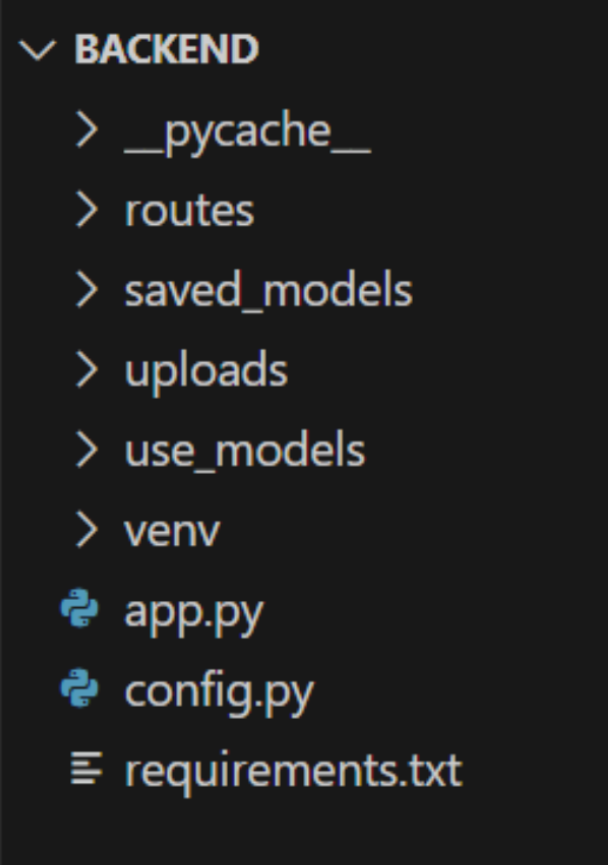
\includegraphics[width=0.9\linewidth]{chapters/chapter56/images/Figure04.png}
        \captionof{figure}{Backend project directory structure.}
        \label{fig:BackendProject}
    \end{minipage}
\end{figure}


\begin{figure}[H]
    \centering
    \begin{minipage}{0.55\textwidth}
        \raggedright
        \textbf{The Frontend includes:}
        \begin{itemize}
            \item \textbf{src/}: Contains all source code for the React application.
            \begin{itemize}
                \item \textbf{assets/}: Directory for static assets such as images or icons.
                \item \textbf{components/}: Contains reusable \gls{abb:ui} components.
                \item \textbf{pages/}: Holds different pages/screens of the application.
                \item \textbf{App.tsx}: Root component that sets up routing and layout.
                \item \textbf{index.css}: Global \gls{abb:css} styles.
                \item \textbf{main.tsx}: Entry point that mounts the React app to the \gls{abb:dom}.
                \item \textbf{vite-env.d.ts}: Type declaration file for Vite.
            \end{itemize}
            \item \textbf{index.html}: Main \gls{abb:html} file used by Vite to render the app.
            \item \textbf{tailwind.config.js}: Tailwind \gls{abb:css} configuration.
            \item \textbf{postcss.config.js}: Configuration for Post\gls{abb:css}.
            \item \textbf{tsconfig.json / tsconfig.node.json}: \gls{abb:ts} compiler settings.
            \item \textbf{vite.config.ts}: Configuration file for the Vite build tool.
            \item \textbf{package.json / package-lock.json}: Manage project dependencies and scripts.
            \item \textbf{.eslintrc.cjs}: ESLint configuration for code quality.
        \end{itemize}
    \end{minipage}%
    \hfill
    \begin{minipage}{0.4\textwidth}
        \centering
        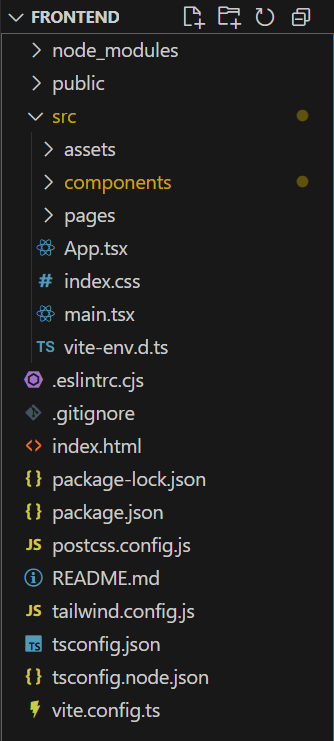
\includegraphics[width=0.9\linewidth]{chapters/chapter56/images/Figure10.png}
        \captionof{figure}{Frontend Project Directory Structure.}
        \label{fig:FrontendProject}
    \end{minipage}
\end{figure}



\subsection{Web platform interfaces}

This section presents the main interfaces of our web application, Wheat Guard, where the models for wheat disease classification and insect pest detection are deployed. Additional interfaces are provided in Appendix\ref{app:annexC}.

\subsubsection{Wheat Disease Detection Interface}
The Wheat Disease Detection Interface (Figure~\ref{fig:uploadImage}) allows users to submit images of wheat crops, perform automated disease detection using trained models, and view classification results with confidence scores. It also highlights infected regions for clearer interpretation (Figure~\ref{fig:WheatDiseaseClassificationpage}).

\begin{figure}[H]
    \centering
    \begin{minipage}{0.48\textwidth}
        \centering
        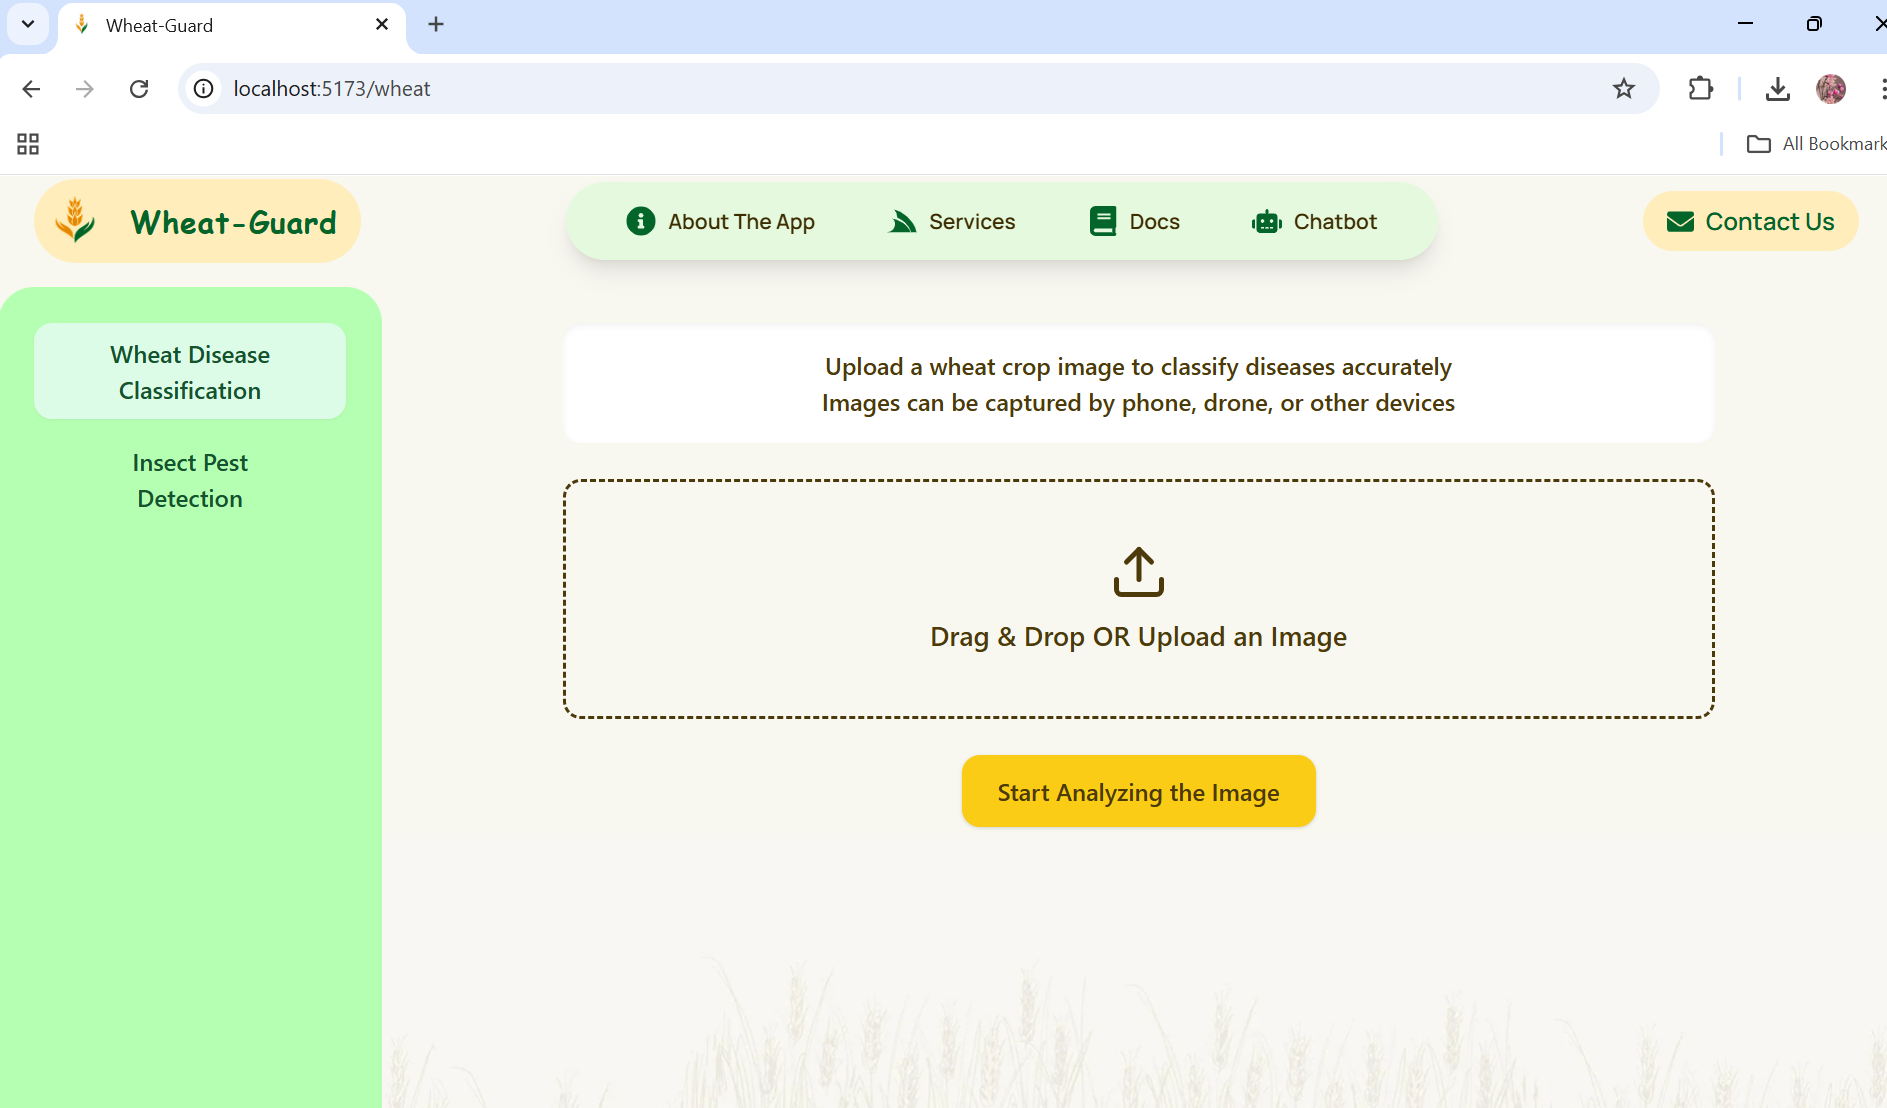
\includegraphics[width=\textwidth]{chapters/chapter56/images/Figure05.png}
        \caption{Upload an image to analyze and detect wheat diseases.}
        \label{fig:uploadImage}
    \end{minipage}
    \hfill
    \begin{minipage}{0.48\textwidth}
        \centering
        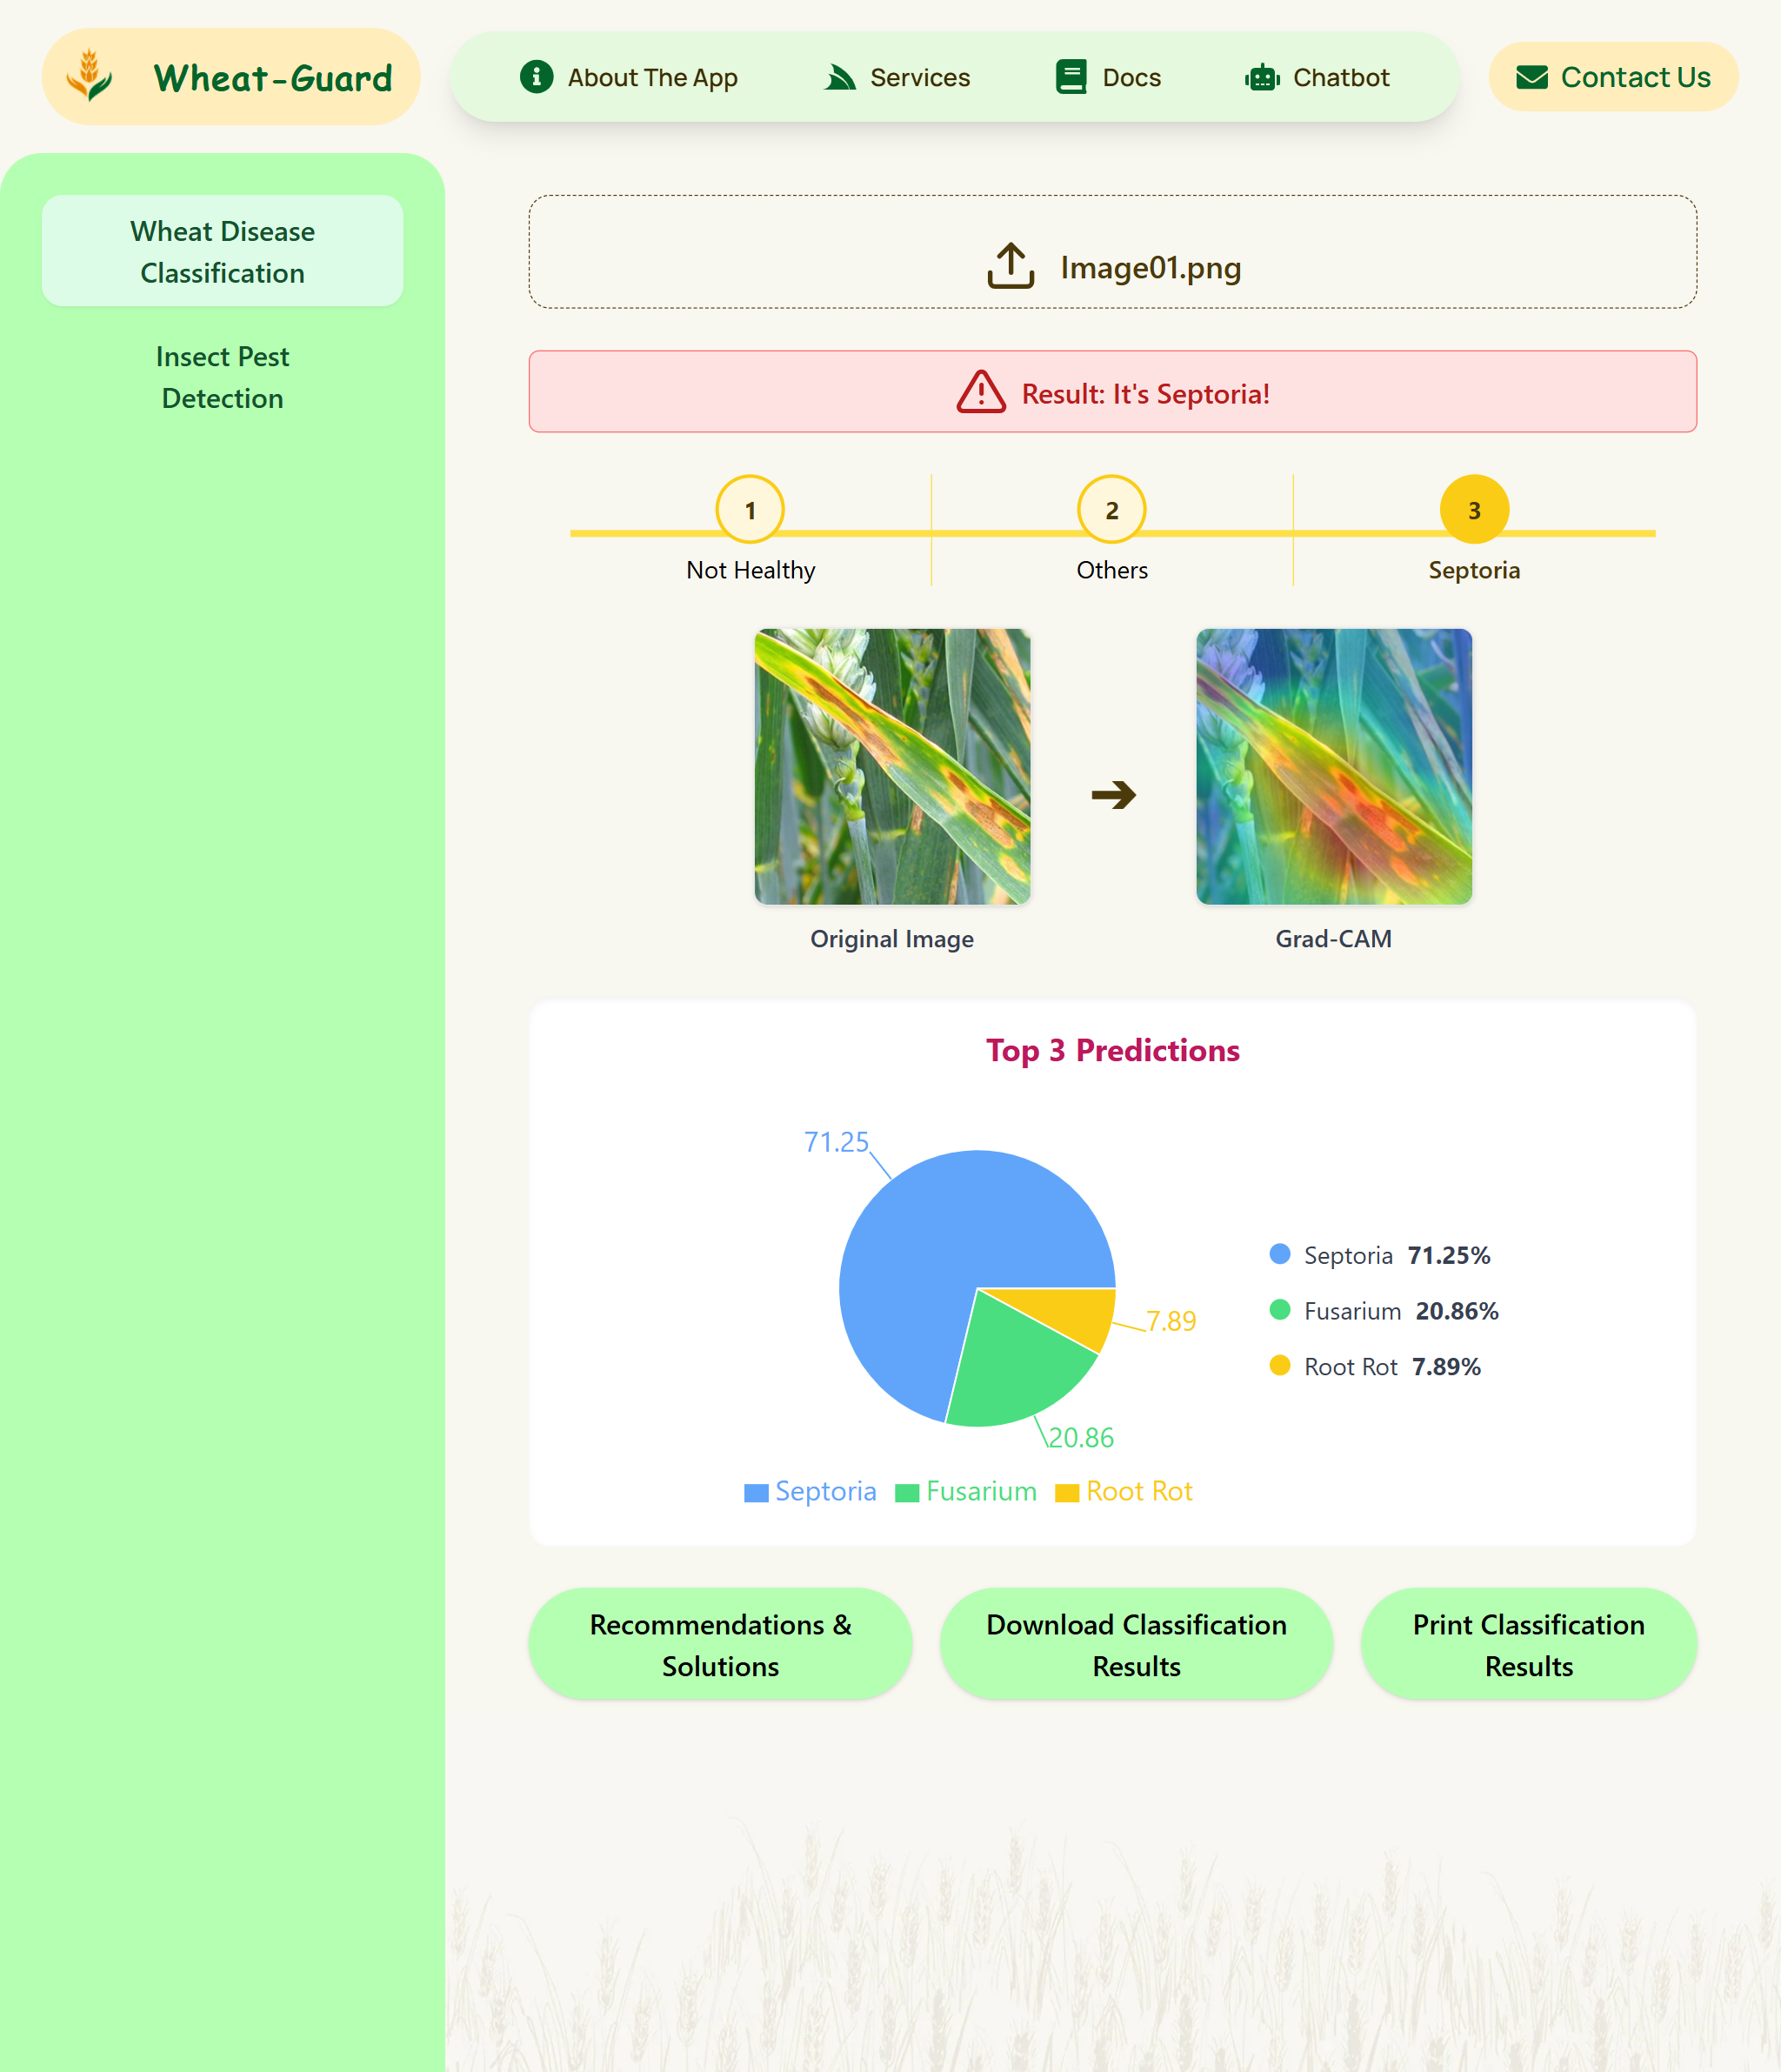
\includegraphics[width=\textwidth]{chapters/chapter56/images/Figure06.png}
        \caption{Wheat disease classification results.}
        \label{fig:WheatDiseaseClassificationpage}
    \end{minipage}
\end{figure}



\subsubsection{Insect pest detection page}

The Insect Pest Detection page (Figure~\ref{fig:Insectpestdetectionpage}) allows users to upload images of wheat crops suspected of pest infestation. The system automatically analyzes the images to identify common insect pests that affect wheat. Users receive detailed detection results along with visual indicators highlighting the regions where pests are detected.

\begin{figure}[H] % 'H' needs \usepackage{float}
    \centering
    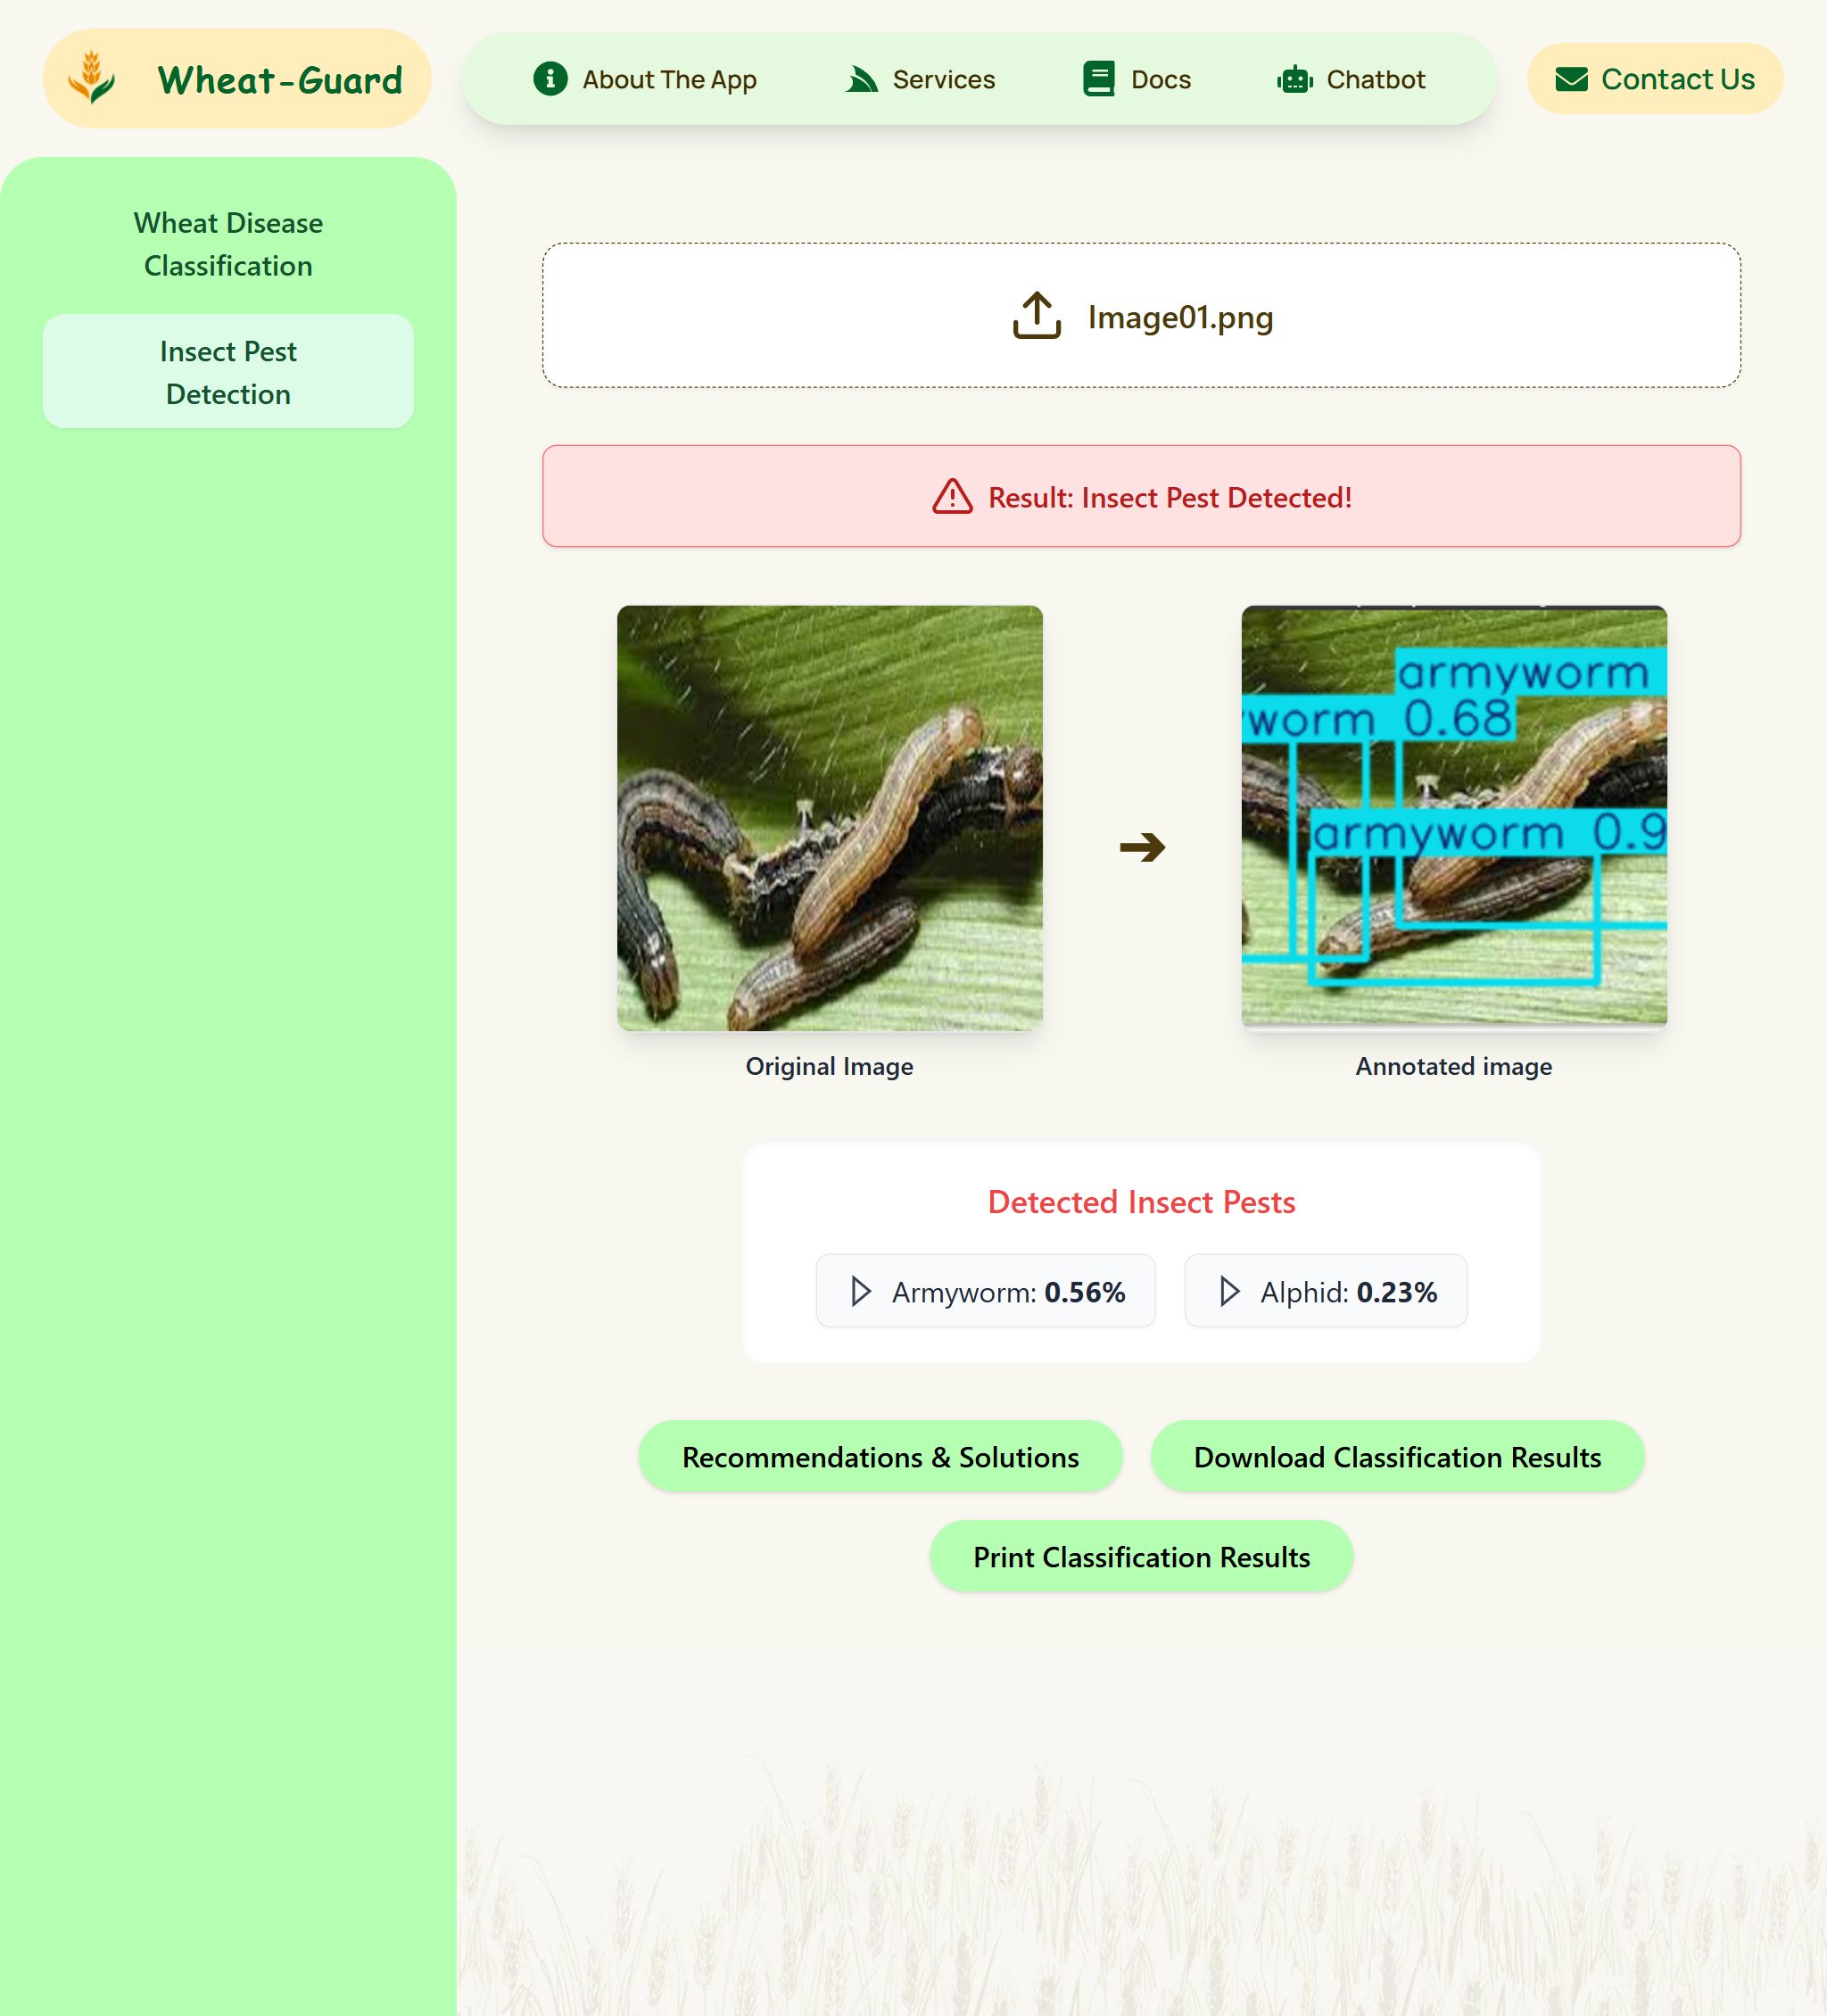
\includegraphics[width=0.7\textwidth]{chapters/chapter56/images/Figure07.png}
    \caption{Insect pest detection page.}
    \label{fig:Insectpestdetectionpage}
\end{figure}


\subsubsection{AI Assistant Page}

The AI Assistant page (Figure~\ref{fig:AIAssistantPage}) is designed to provide users with a conversational interface for interactive support. Users can either send a message or upload an image to ask questions related to wheat diseases and pest control. The assistant leverages an integrated natural language processing model to deliver informative and context-aware responses, making the platform more accessible and user-friendly, especially for non-experts in agriculture or technology.

\begin{figure}[H] % 'H' needs \usepackage{float}
    \centering
    
\includegraphics[width=0.8\textwidth]{chapters/chapter5/images/Figure11.png}
    \caption{AI Assistant page interface.}
    \label{fig:AIAssistantPage}
\end{figure}

% -----------------------------Test-------------------------------
\section{Evaluation metrics}

We used several widely recognized evaluation metrics to assess our classification models' performance. These metrics help quantify the models' effectiveness in correctly identifying and classifying wheat diseases and insect pests.

A confusion matrix is a tabular representation of the actual versus predicted classifications. It provides a comprehensive view of model performance across all classes, showing true positives (TP), true negatives (TN), false positives (FP), and false negatives (FN) for each class.

\begin{itemize}
    \item \textbf{Accuracy:} Measures the proportion of correct predictions (both true positives and true negatives) among the total number of predictions, as shown in Equation~\ref{eq:accuracy}.
    \begin{equation}
        \text{Accuracy} = \frac{TP + TN}{TP + TN + FP + FN}
        \label{eq:accuracy}
    \end{equation}

    \item \textbf{Precision:} Indicates the proportion of correctly predicted positive observations to the total predicted positives. It is useful when the cost of false positives is high (Equation~\ref{eq:precision}).
    \begin{equation}
        \text{Precision} = \frac{TP}{TP + FP}
        \label{eq:precision}
    \end{equation}

    \item \textbf{Recall:} Measures the proportion of correctly predicted positive observations out of all actual positives. It is important when the cost of false negatives is high (Equation~\ref{eq:recall}).
    \begin{equation}
        \text{Recall} = \frac{TP}{TP + FN}
        \label{eq:recall}
    \end{equation}

    \item \textbf{F1-score:} The harmonic mean of precision and recall. It balances the two, especially when the class distribution is uneven (Equation~\ref{eq:f1score}).
    \begin{equation}
        \text{F1-score} = 2 \cdot \frac{\text{Precision} \cdot \text{Recall}}{\text{Precision} + \text{Recall}}
        \label{eq:f1score}
    \end{equation}
\end{itemize}

For the insect pest detection task, we considered several widely adopted evaluation metrics in object detection:

\begin{itemize}
    \item \textbf{Intersection over Union (IoU)} is a fundamental metric used to evaluate the overlap between predicted and ground-truth bounding boxes. It is defined as the ratio of the area of intersection to the area of union between the predicted box ($B_p$) and the ground-truth box ($B_{gt}$):

    \begin{equation}
        \text{IoU} = \frac{\text{Area}(B_p \cap B_{gt})}{\text{Area}(B_p \cup B_{gt})}
    \end{equation}

    A prediction is typically considered correct if the IoU exceeds a predefined threshold, such as 0.5.

    
    \item \textbf{Mean Average Precision (mAP)} is a key metric that evaluates the balance between precision and recall across various confidence thresholds.

    The \textbf{Average Precision (AP)} for a single class is defined as the area under the Precision–Recall (P–R) curve:

    \begin{equation}
        \text{AP} = \int_{0}^{1} \text{Precision}(\text{Recall}) \, d(\text{Recall})
    \end{equation}

    The \textbf{Mean Average Precision (mAP)} is the mean of the AP values over all $n$ object categories:

    \begin{equation}
        \text{mAP} = \frac{1}{n} \sum_{i=1}^{n} \text{AP}_i
    \end{equation}

    In the special case of a single-category task ($n = 1$), mAP is equivalent to the AP of that category.

    Common mAP variants include:
    \begin{itemize}
        \item \textbf{mAP@0.5}: Average Precision computed using an Intersection over Union (IoU) threshold of 0.5.
        \item \textbf{mAP@0.5:0.95}: Mean AP computed across multiple IoU thresholds ranging from 0.5 to 0.95 (with a step size of 0.05), offering a more comprehensive evaluation.
    \end{itemize}

    \item \textbf{Mean Precision} evaluates the proportion of correct positive predictions across all $C$ classes. It is calculated as:

    \begin{equation}
        \text{Mean Precision} = \frac{1}{C} \sum_{i=1}^{C} \frac{TP_i}{TP_i + FP_i}
    \end{equation}

    where $TP_i$ and $FP_i$ denote the number of true positives and false positives for class $i$, respectively.

    \item \textbf{Mean Recall} measures the model’s ability to correctly identify all relevant instances across all classes. It is defined as:

    \begin{equation}
        \text{Mean Recall} = \frac{1}{C} \sum_{i=1}^{C} \frac{TP_i}{TP_i + FN_i}
    \end{equation}

    where $FN_i$ is the number of false negatives for class $i$.
    
\end{itemize}


These metrics provide a holistic evaluation of the model's ability to classify and detect both wheat diseases and insect pests effectively in real-world conditions.



\section{Objectives of the experiments}

The main objective of our experiments is to justify the choices made during the design and implementation of our system. This includes evaluating the different CNN architectures used, as well as the selection of optimizers and technologies such as attention mechanisms. Each component was chosen based on its potential to enhance the model’s performance in detecting and classifying wheat diseases.

Moreover, we aim to prove the effectiveness of the hierarchical classification approach, which is central to our system. By conducting various tests and comparisons, we seek to assess how this approach performs under different configurations and against alternative strategies.

Finally, we compare our proposed solution with existing state-of-the-art methods by re-implementing these approaches on our dataset. This allows us to rigorously evaluate the relative performance and demonstrate the superiority and robustness of our system in a fair and consistent setting.


\section{Experimental results in wheat disease classification models}

We defined two distinct test scenarios to evaluate our system. The first scenario focuses on testing the binary classification model, which is designed to classify whether a given sample is healthy or diseased. The second scenario evaluates the multiclass classification mode to identify the specific disease category affecting the sample.

\subsection{Scenario 1: Justification of the Architecture Selection for the Binary Classification Model}
\label{sec:testcnnModel1}
In this scenario, we will investigate the performance of multiple CNN architectures as feature extractors and assess their integration with a range of traditional machine learning classifiers to determine the most effective combinations for our task.
\subsubsection{Testing different CNN architectures for feature extraction}
This section explores the effectiveness of various pretrained convolutional neural network (CNN) architectures for image feature extraction. By evaluating the quality of extracted features using unsupervised clustering metrics, the goal is to identify models that best capture discriminative patterns while balancing accuracy, dimensionality, and computational cost.

\paragraph{Load and preprocess the dataset:}  
The dataset D1 is prepared by normalizing image pixel values to a [0, 1] scale, selecting 80\% of the data for training, and loading this subset in a fixed order to maintain the correct association between images and their labels during feature extraction. Additionally, the D1 dataset was augmented using a combination of techniques, including gamma correction, CutOut, Mixup, and CutMix.

\paragraph{Define pretrained CNN architectures:}  
A set of pretrained CNN architectures, such as EfficientNetB2, MobileNet, VGG19, Xception, InceptionV3, DenseNet169, DenseNet201, ResNet50V2, and ResNet101V2, all trained on the ImageNet dataset, are used as feature extractors. These models are applied without their original classification layers and fixed during evaluation to ensure they only generate feature representations. The model outputs a one-dimensional feature vector for each input image using global average pooling, capturing the most relevant high-level information from the image.

\paragraph{Extract features and evaluate feature quality using clustering metrics:}  
Deep features are extracted from each image in the training set using the selected CNN architectures. The resulting feature vectors, along with their corresponding class labels, are collected for further analysis.

To evaluate the discriminative power of these features without relying on a supervised classifier, two unsupervised clustering metrics are employed:

\begin{itemize}
    \item \textbf{Silhouette Score}:  
    The Silhouette Score combines cohesion (how close a point is to others in the same class) and separation (how far it is from points in other classes). For a single sample $i$, the silhouette coefficient is calculated as shown in Equation~\ref{eq:silhouette}:
    \begin{equation}
        s(i) = \frac{b(i) - a(i)}{\max(a(i), b(i))}
        \label{eq:silhouette}
    \end{equation}
    where $a(i)$ is the average distance to other points in the same class, and $b(i)$ is the minimum average distance to points in a different class. The score ranges from $-1$ to $1$, with values closer to $1$ indicating well-clustered data.

    \item \textbf{Davies–Bouldin Score (DBI)}:  
    The Davies–Bouldin Score evaluates intra-cluster similarity relative to inter-cluster differences. It is calculated as shown in Equation~\ref{eq:dbi}:
    \begin{equation}
        \text{DBI} = \frac{1}{n} \sum_{i=1}^{n} \max_{j \neq i} \left( \frac{\sigma_i + \sigma_j}{d_{ij}} \right)
        \label{eq:dbi}
    \end{equation}
    where $\sigma_i$ is the average distance between each point in cluster $i$ and the centroid of that cluster, and $d_{ij}$ is the distance between the centroids of clusters $i$ and $j$. Lower DBI values indicate better separation and more compact clusters.
\end{itemize}


\paragraph{Compare and summarize results:}  
Table~\ref{tab:cnn_comparison_res} presents the results of applying various pre-trained CNN architectures for feature extraction. Based on the comparison, the three best-performing models are EfficientNetB2, VGG19, and DenseNet169.

\begin{itemize}
    \item \textbf{EfficientNetB2} achieved the highest silhouette score (0.034) and a reasonable extraction time (38.14 s) with moderate feature dimensionality (1408), making it a strong candidate for capturing discriminative features while maintaining computational efficiency.

    \item \textbf{VGG19}, despite its longer processing time (112.41 s), produced the lowest DB score (6.368) and the smallest feature dimension (512), indicating highly compact and well-separated feature representations suitable for clustering.

    \item \textbf{DenseNet169} also showed competitive clustering performance with a silhouette score of 0.020, a DB score of 6.739, an acceptable dimensionality (1664), and moderate time cost (53.28 s), offering a good balance between quality and efficiency.
\end{itemize}

These models were selected for their ability to extract informative and discriminative features while maintaining trade-offs between accuracy, compactness, and processing time.


% \begin{figure}[H] % 'H' needs \usepackage{float}
%     \centering
%     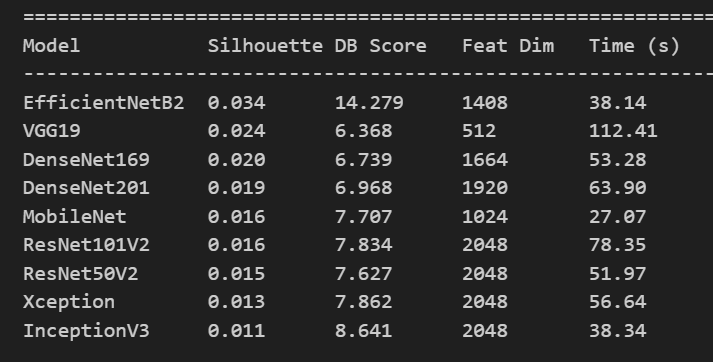
\includegraphics[width=0.9\textwidth]{chapters/chapter56/images/Figure01.png}
%     \caption{ Performance comparison of pre-trained CNN architectures for feature extraction based on clustering metrics, feature dimensionality, and extraction time.}
%     \label{fig:cnn-results}
% \end{figure}

\begin{table}[h!]
\centering
\begin{tabular}{|l|c|c|c|c|}
\hline
\textbf{Model} & \textbf{Silhouette} & \textbf{DB Score} & \textbf{Feat Dim} & \textbf{Time (s)} \\
\hline
EfficientNetB2 & 0.034 & 14.279 & 1408 & 38.14 \\
VGG19          & 0.024 & 6.368  & 512  & 112.41 \\
DenseNet169    & 0.020 & 6.739  & 1664 & 53.28 \\
DenseNet201    & 0.019 & 6.968  & 1920 & 63.90 \\
MobileNet      & 0.016 & 7.707  & 1024 & 27.07 \\
ResNet101V2    & 0.016 & 7.834  & 2048 & 78.35 \\
ResNet50V2     & 0.015 & 7.627  & 2048 & 51.97 \\
Xception       & 0.013 & 7.862  & 2048 & 56.64 \\
InceptionV3    & 0.011 & 8.641  & 2048 & 38.34 \\
\hline
\end{tabular}
\caption{Comparison of different CNN models based on clustering performance and feature extraction time.}
\label{tab:cnn_comparison_res}
\end{table}







\subsubsection{Testing different machine learning models for classification}
\label{sec:MLclassifiertest}

In this experiment, EfficientNetB2, VGG19, and DenseNet169 were selected as the feature extractors, based on their strong performance in the previous evaluation. Features extracted from each CNN were then used to train and evaluate multiple machine learning classifiers for binary classification: Decision Tree (DT), Random Forest (RF), Support Vector Machine (SVM), and Multi-Layer Perceptron (MLP). A comprehensive grid search was performed to optimize the hyperparameters of each classifier (as detailed in Table~\ref{tab:hyperparams}). The models were assessed using standard classification metrics, including accuracy, recall, precision, and F1-score (see Table~\ref{tab:performance}). Among the evaluated classifiers, the SVM achieved the best overall performance, demonstrating its effectiveness in leveraging the extracted features for accurate classification.

\begin{table}[H]
    \centering
    \renewcommand{\arraystretch}{1.5}
    \setlength{\tabcolsep}{8pt}
    \caption{\textit{Classifier hyperparameter grid search.}}
    \label{tab:hyperparams}
    \begin{tabular}{|p{1.5cm}|p{5.2cm}|p{5.3cm}|}
        \hline
        \textbf{Classifier} & \textbf{Hyperparameter} & \textbf{Explored Values} \\ \hline

        \multirow{4}{*}{SVM} 
        & Regularization parameter ($C$) & \{0.1, 1, 10\} \\ \cline{2-3}
        & Kernel type & \{linear, rbf, poly\} \\ \cline{2-3}
        & Kernel coefficient ($\gamma$) & \{scale, auto\} \\ \cline{2-3}
        & Polynomial degree (for poly kernel) & \{2, 3, 4\} \\ \hline

        \multirow{4}{*}{MLP} 
        & Hidden layer sizes & (50), (100), (100, 50) \\ \cline{2-3}
        & Activation function & \{ReLU, tanh\} \\ \cline{2-3}
        & Optimizer & \{adam, sgd\} \\ \cline{2-3}
        & Learning rate strategy & \{constant, adaptive\} \\ \hline

        \multirow{4}{*}{RF} 
        & Number of estimators & \{50, 100, 200\} \\ \cline{2-3}
        & Max features & \{sqrt, log2\} \\ \cline{2-3}
        & Min samples per leaf & \{1, 2, 5\} \\ \cline{2-3}
        & Min samples to split & \{2, 5, 10\} \\ \hline

        \multirow{3}{*}{DT} 
        & Maximum depth & \{50, 100, 200\} \\ \cline{2-3}
        & Split criterion & \{gini, entropy\} \\ \cline{2-3}
        & Min samples per leaf & \{1, 2, 5\} \\ \hline
    \end{tabular}
\end{table}



\vspace{1cm}

\begin{table}[H]
    \centering
    \renewcommand{\arraystretch}{1.4}
    \setlength{\tabcolsep}{10pt}
    \caption{Performance of machine learning classifiers using CNN feature extraction on the augmented D1 dataset.}
    \label{tab:performance}
    \begin{tabular}{|p{2.5cm}|p{4cm}|c|c|c|c|}
        \hline
        \textbf{Dataset} & \textbf{Classifier} & \textbf{Accuracy} & \textbf{Recall} & \textbf{Precision} & \textbf{F1-Score} \\ \hline
        
        \multirow{4}{*}{Augmented D1} 
        & Random Forest (RF) & 0.9867 & 0.9852 & 0.9880 & 0.9865 \\ \cline{2-6}
        & Decision Tree (DT) & 0.9547 & 0.9553 & 0.9534 & 0.9543 \\ \cline{2-6}
        & Support Vector Machine (SVM) & \textbf{0.9960} & \textbf{0.9958} & \textbf{0.9961} & \textbf{0.9960} \\ \cline{2-6}
        & Multilayer Perceptron (MLP) & 0.9940 & 0.9940 & 0.9939 & 0.9939 \\ \hline
    \end{tabular}
\end{table}





\subsection{Scenario 2: Justification of the Architecture Selection for the multiclass disease classification model}
This scenario involves testing \gls{abb:cnn} architectures with optimizers (Stochastic Gradient Descent (SGD) and Adaptive Moment Estimation (ADAM)) for feature extraction and examining the effect of different attention mechanisms on multiclass disease classification.

\subsubsection{Testing different CNN architectures with optimizers for feature extraction}
\label{sec:TestCnnM2}
In this experiment, we systematically evaluated the influence of various convolutional neural network (CNN) architectures combined with different optimization algorithms on the performance of multiclass classification tasks. We utilized CNNs not only for feature extraction but also for the end-to-end classification process, allowing the networks to learn both robust feature representations and decision boundaries simultaneously. The dataset employed, referred to as D2, incorporated extensive data augmentation techniques as described in Section~\ref{sec:data_augmentation}, which helped improve model generalization by increasing the diversity of the training samples.

For each CNN architecture, we tested two widely used optimizers, SGD and Adam, to analyze how the choice of optimization strategy affects the training dynamics and final model accuracy. Model performance was rigorously evaluated using four key metrics: accuracy, recall, precision, and F1-score, providing a comprehensive understanding of classification effectiveness from multiple perspectives, including overall correctness, sensitivity to positive classes, and balance between precision and recall.

The experiments were conducted using consistent training settings, outlined in Table~\ref{tab:hyperparameters}, to ensure fair comparison between different models.

\begin{table}[H]
    \centering
    \caption{Training hyperparameters used for CNN evaluation.}
    \label{tab:hyperparameters}
    \renewcommand{\arraystretch}{1.4}
    \begin{tabular}{|p{5.5cm}|p{8cm}|}
        \hline
        \textbf{Hyperparameter} & \textbf{Value} \\ \hline
        Optimizers Tested & Stochastic Gradient Descent (momentum = 0.9, weight decay = 0.00001), Adam \\ \hline
        Initial Learning Rate & 0.001 \\ \hline
        Learning Rate Scheduler & Cosine Annealing Learning Rate (maximum iterations = 25, minimum learning rate = 0.00001) \\ \hline
        Loss Function & Cross-Entropy Loss with label smoothing factor = 0.1 \\ \hline
        Batch Size & 16 \\ \hline
        Input Image Size & 448 $\times$ 448 pixels \\ \hline
        Dropout Rate & 0.3 \\ \hline
        Number of Training Epochs & 25 \\ \hline
        Data Augmentation Techniques & Resize, Random Crop, Horizontal Flip, Random 90-degree Rotation, Shift-Scale-Rotate, Hue-Saturation-Value Adjustment, Random Brightness and Contrast, Gaussian Blur, Normalization, MixUp, CutMix, Cutout, Gamma Correction \\ \hline
    \end{tabular}
\end{table}

As summarized in Table~\ref{tab:cnn_performance}, the ResNet50V2 architecture coupled with the SGD optimizer consistently delivered superior results, achieving an accuracy of 99.25\%, a recall of 99.35\%, a precision of 98.80\%, and an F1-score of 99.04\%. These results indicate that this combination is highly effective at extracting discriminative features that enable the model to distinguish between classes with remarkable precision and reliability.

\begin{table}[H]
    \centering
    \renewcommand{\arraystretch}{1.4}
    \setlength{\tabcolsep}{10pt}
    \caption{Classification performance of CNN architectures using SGD and Adam optimizers.}
    \label{tab:cnn_performance}
    \begin{tabular}{|p{4cm}|p{2cm}|c|c|c|c|}
        \hline
        \textbf{CNN Architecture} & \textbf{Optimizer} & \textbf{Accuracy} & \textbf{Recall} & \textbf{Precision} & \textbf{F1-Score} \\ \hline

        \multirow{2}{*}{EfficientNetB2} 
        & SGD  & 96.57\% & 95.54\% & 94.34\% & 94.73\% \\ \cline{2-6}
        & Adam & 98.10\% & 96.94\% & 97.51\% & 97.22\% \\ \hline

        \multirow{2}{*}{MobileNet} 
        & SGD  & 94.29\% & 90.87\% & 94.14\% & 91.97\% \\ \cline{2-6}
        & Adam & 95.81\% & 94.02\% & 94.98\% & 94.45\% \\ \hline

        \multirow{2}{*}{Xception} 
        & SGD  & 96.99\% & 96.16\% & 96.40\% & 96.25\% \\ \cline{2-6}
        & Adam & 96.61\% & 94.11\% & 95.77\% & 94.86\% \\ \hline

        \multirow{2}{*}{InceptionV3} 
        & SGD  & 97.90\% & 97.47\% & 98.19\% & 97.81\% \\ \cline{2-6}
        & Adam & 92.38\% & 93.43\% & 89.91\% & 91.05\% \\ \hline

        \multirow{2}{*}{DenseNet201} 
        & SGD  & 98.87\% & 97.99\% & 98.43\% & 98.19\% \\ \cline{2-6}
        & Adam & 95.86\% & 94.87\% & 95.13\% & 94.97\% \\ \hline

        \multirow{2}{*}{ResNet50V2} 
        & SGD  & \textbf{99.25\%} & \textbf{99.35\%} & \textbf{98.80\%} & \textbf{99.04\%} \\ \cline{2-6}
        & Adam & 92.28\% & 89.67\% & 92.27\% & 90.57\% \\ \hline
    \end{tabular}
\end{table}

\vspace{0.5cm}




\subsubsection{Testing different attention mechanisms}
\label{sec:attentionMecanisme}
Building on the results obtained from the previous experiment, where the ResNet50V2 architecture combined with the Stochastic Gradient Descent (SGD) optimizer achieved the best overall performance, we selected this configuration as the baseline for further enhancement.

To further improve the classification performance, particularly in capturing subtle inter-class variations, we extended our investigation by integrating various attention mechanisms into the ResNet50V2 backbone. This experiment aims to evaluate the impact of spatial and channel-wise attention on the model’s capacity to prioritize informative regions in feature maps. Specifically, we examined four widely adopted attention modules: Self-Attention, Squeeze-and-Excitation (SE), Convolutional Block Attention Module (CBAM), and Efficient Channel Attention (ECA). Each of these mechanisms is designed to guide the network’s focus toward the most relevant features, thereby enhancing representational power and ultimately classification accuracy.

The theoretical background and functional details of the attention modules including their architectural designs and integration strategies are provided in Appendix\ref{app:annexA}.


\begin{table}[h!]
\centering
\caption{Performance comparison of attention mechanisms.}
\label{tab:attention_mechanisms}
\begin{tabular}{|c|c|c|c|c|}
\hline
\textbf{Attention Mechanism} & \textbf{Test Accuracy} & \textbf{Recall} & \textbf{Precision} & \textbf{F1 Score} \\
\hline
Self-Attention              & 99.83\% & 99.77\% & 99.78\% & 99.79\% \\
\hline
SE (Squeeze-and-Excitation)& 99.81\% & 99.76\% & 99.77\% & 99.79\% \\
\hline
CBAM                       & 99.75\% & 99.69\% & 99.68\% & 99.70\% \\
\hline
ECA                        & \textbf{99.83\%} & \textbf{99.78\%} & \textbf{99.79\%} & \textbf{99.81\%} \\
\hline
\end{tabular}
\end{table}

\vspace{0.5cm}

On the augmented D2 dataset, the model incorporating the Efficient Channel Attention (ECA) mechanism delivered the best overall performance across all evaluation metrics, as shown in Table~\ref{tab:attention_mechanisms}, demonstrating its ability to enhance feature representations and improve classification accuracy effectively. Not far behind, the model integrated with the Self-Attention mechanism achieved similarly strong and balanced results, reflecting its capacity to capture long-range dependencies between features. 

This is further illustrated in Figure~\ref{fig:confusion_matrix}, which presents the confusion matrix for the ResNet50 model enhanced with the ECA attention mechanism, highlighting its strong ability to distinguish between classes with minimal misclassifications.

\begin{figure}[h!]
\centering
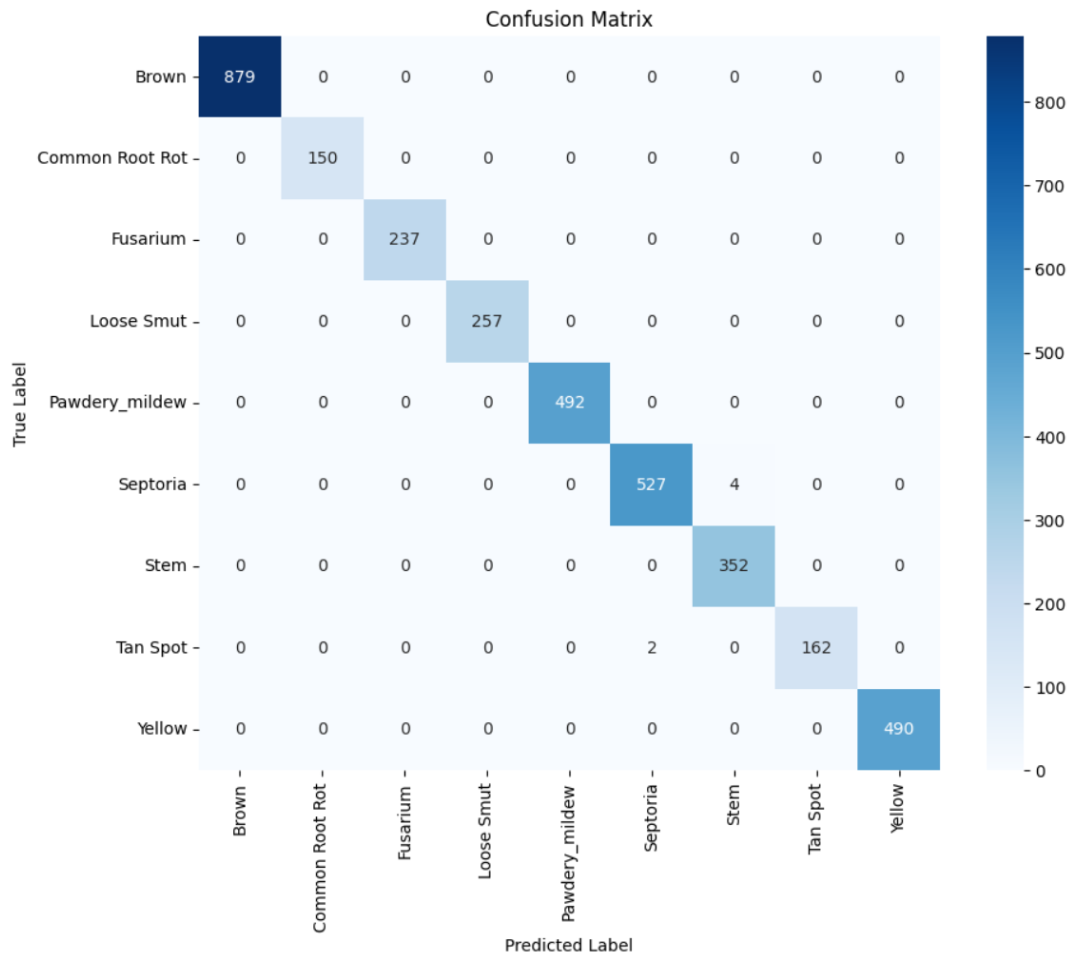
\includegraphics[width=0.9\textwidth]{chapters/chapter56/images/Figure02.png}
\caption{Confusion matrix of the multiclass classification model (M2).}
\label{fig:confusion_matrix}
\end{figure}


\textbf{Grad-CAM visualization} \\

To gain deeper insight into how different attention mechanisms influence the model’s decision-making process, we employed Grad-CAM (Gradient-weighted Class Activation Mapping). This technique provides visual explanations by highlighting the most relevant regions of the input image that contribute to the final prediction.

Grad-CAM works by using the gradients of the target class flowing into the final convolutional layer to generate a coarse localization map of the important regions in the image. We chose the output of the last convolutional stage for generating these attention maps because fully connected layers discard spatial information, while deeper convolutional layers retain both spatial and high-level semantic information. This makes them ideal for producing class-discriminative visual explanations.

The effectiveness of different attention mechanisms is illustrated in Figure~\ref{fig:grad_cam}, showing how each module, SE (Squeeze-and-Excitation), CBAM (Convolutional Block Attention Module), ECA (Efficient Channel Attention), and Self-Attention, directs the model’s focus toward the most informative areas of the input image. These visualizations confirm that integrating attention modules improves the model’s ability to capture and utilize critical features for accurate classification.

\begin{figure}[h!]
\centering
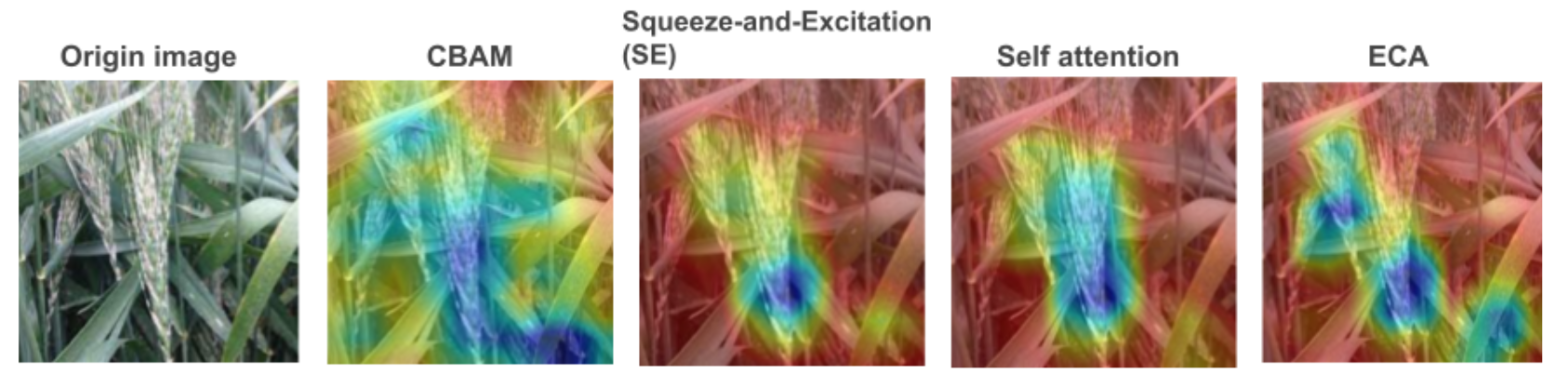
\includegraphics[width=0.9\textwidth]{chapters/chapter56/images/Figure03.png}
\caption{Grad-CAM Visualization of Different Attention Mechanisms: SE, CBAM, ECA, and Self-Attention.}
\label{fig:grad_cam}
\end{figure}


\section{The performance of the hierarchical classification approach}
\label{sec:justifyHAmodel}

In our work, we deliberately chose a hierarchical classification framework over a single multi-class model for several important technical and performance related reasons.

Firstly, attempting to use a single model to classify all ten classes distinguishing between healthy plants and nine disease categories presented significant challenges. Specifically, integrating Model 1 into a full-scale multi-class setting led to memory overflow issues. The SVM component, in particular, does not scale well when dealing with large, complex multi-class feature spaces extracted from deep CNNs. Its performance degrades considerably and becomes computationally infeasible on our hardware setup.

Secondly, we explored an alternative approach by applying Model 2 directly to predict all ten classes in a flat manner, including the healthy class. This model was evaluated using 20\% of the global dataset and achieved an overall accuracy of 98.99\% (Table~\ref{tab:single-hierarchical}). However, its performance on the “healthy” class was noticeably poor. As illustrated in Figure~\ref{fig:confusion_matrics_single_model}, there was a significant rate of false positives, where healthy samples were frequently misclassified as diseased. This is highly undesirable in a real-world agricultural setting, as it can lead to false alarms and unnecessary interventions.


\begin{table}[H]
\centering
\renewcommand{\arraystretch}{1.3}
\setlength{\tabcolsep}{6pt}
\caption{Performance comparison of individual and hierarchical classification strategies}
\begin{tabular}{|p{3.5cm}|p{3.7cm}|p{1.9cm}|p{1.9cm}|p{1.9cm}|p{1.9cm}|}
\hline
\textbf{Model} & \textbf{Classification Scope} & \textbf{Accuracy (\%)} & \textbf{Recall (\%)} & \textbf{Precision (\%)} & \textbf{F1-score (\%)} \\
\hline
Model 2 (All classes) & 10 classes (Healthy + 9 diseases) & 98.99 & 98.99 & 99.00 & 98.98 \\
\hline
Hierarchical Approach & 10 classes (Model 1 + Model 2) & \textbf{99.48} & \textbf{99.18} & \textbf{99.29} & \textbf{99.31} \\
\hline
\end{tabular}
\label{tab:single-hierarchical}
\end{table}



In contrast, our hierarchical approach effectively mitigates these issues by decomposing the problem into two manageable sub-tasks:

\begin{itemize}
\item \textbf{Model 1} performs a robust binary classification (Healthy vs. Not Healthy), achieving \textbf{99.60\%} accuracy.
\item \textbf{Model 2} then classifies the diseased samples into one of the nine specific disease categories, achieving \textbf{99.83\%} accuracy.
\end{itemize}

The full hierarchical system evaluated on the same 20\% test portion of the global dataset achieved an overall accuracy of \textbf{99.48\%}. This two-stage decomposition not only improves interpretability but also ensures better resource management and enhanced precision in distinguishing healthy cases.

All performance metrics are summarized in Table~\ref{tab:hierarchical}, clearly demonstrating that the hierarchical approach outperforms the conventional multi-class alternative, particularly in minimizing false positives and maintaining high accuracy across all classes. These improvements are further illustrated in the confusion matrix shown in Figure~\ref{fig:confusion_hierarchical}, which highlights the model’s ability to significantly reduce misclassification of healthy samples.



\begin{table}[H]
\centering
\renewcommand{\arraystretch}{1.3}
\setlength{\tabcolsep}{6pt}
\caption{Performance Summary of the Hierarchical Classification Approach}
\begin{tabular}{|p{3.5cm}|p{3.7cm}|p{1.9cm}|p{1.9cm}|p{1.9cm}|p{1.9cm}|}
\hline
\textbf{Model} & \textbf{Classification Scope} & \textbf{Accuracy (\%)} & \textbf{Recall (\%)} & \textbf{Precision (\%)} & \textbf{F1-score (\%)} \\
\hline
Model 1 (Binary) & 2 classes (Healthy / Not Healthy) & 99.60 & 99.58 & 99.59 & 99.60 \\
\hline
Model 2 (Diseases only) & 9 classes (given Not Healthy) & 99.83 & 99.78 & 99.79 & 99.81 \\
\hline
Hierarchical Approach & 10 classes (Model 1 + Model 2) & 99.48 & 99.18 & 99.29 & 99.31 \\
\hline
\end{tabular}
\label{tab:hierarchical}
\end{table}









\vspace{0.5cm} % optional

\begin{figure}[H]
\centering
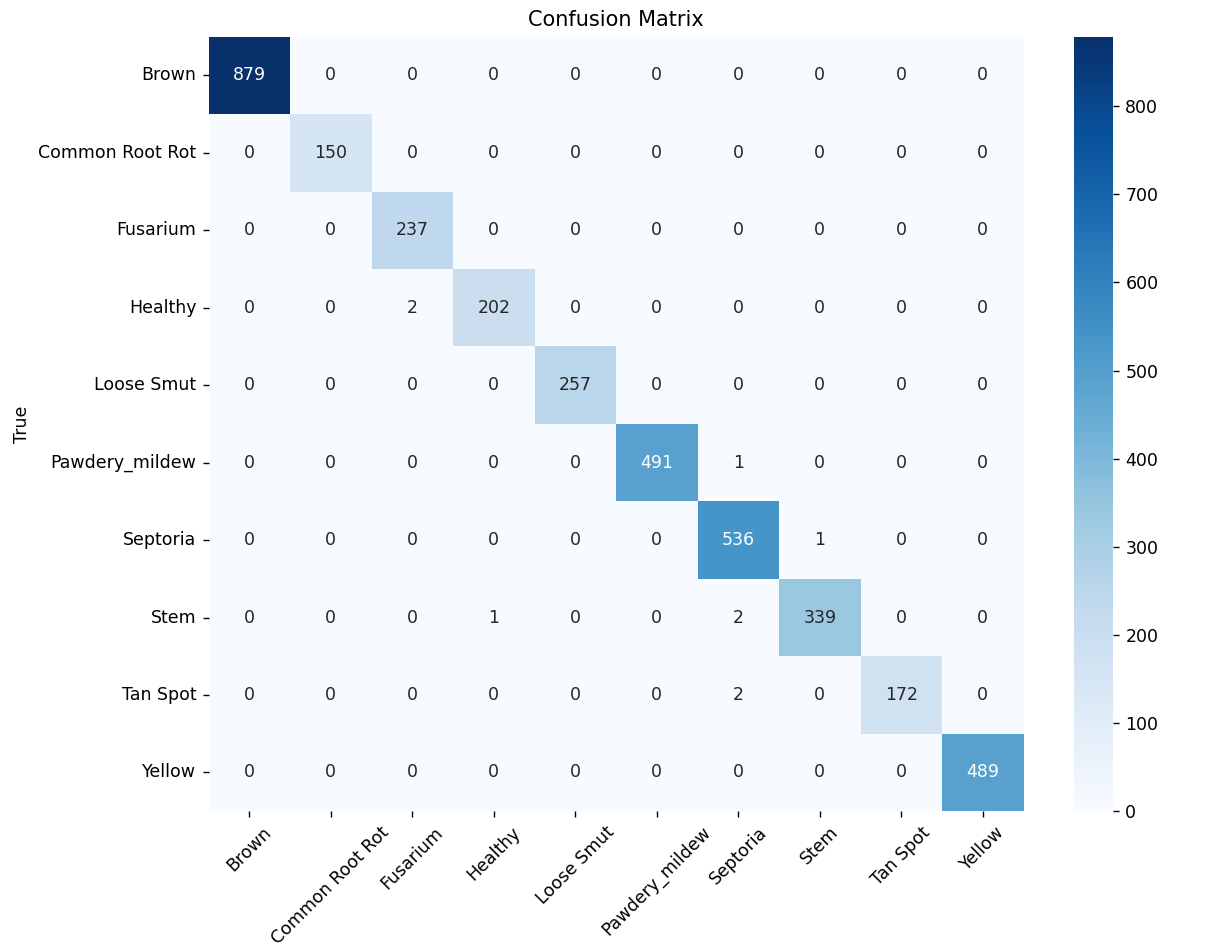
\includegraphics[width=0.8\textwidth]{chapters/chapter56/images/Figure004.png}
\caption{Confusion Matrix of the Hierarchical Classification System.}
\label{fig:confusion_hierarchical}
\end{figure}



\begin{figure}[H]
\centering
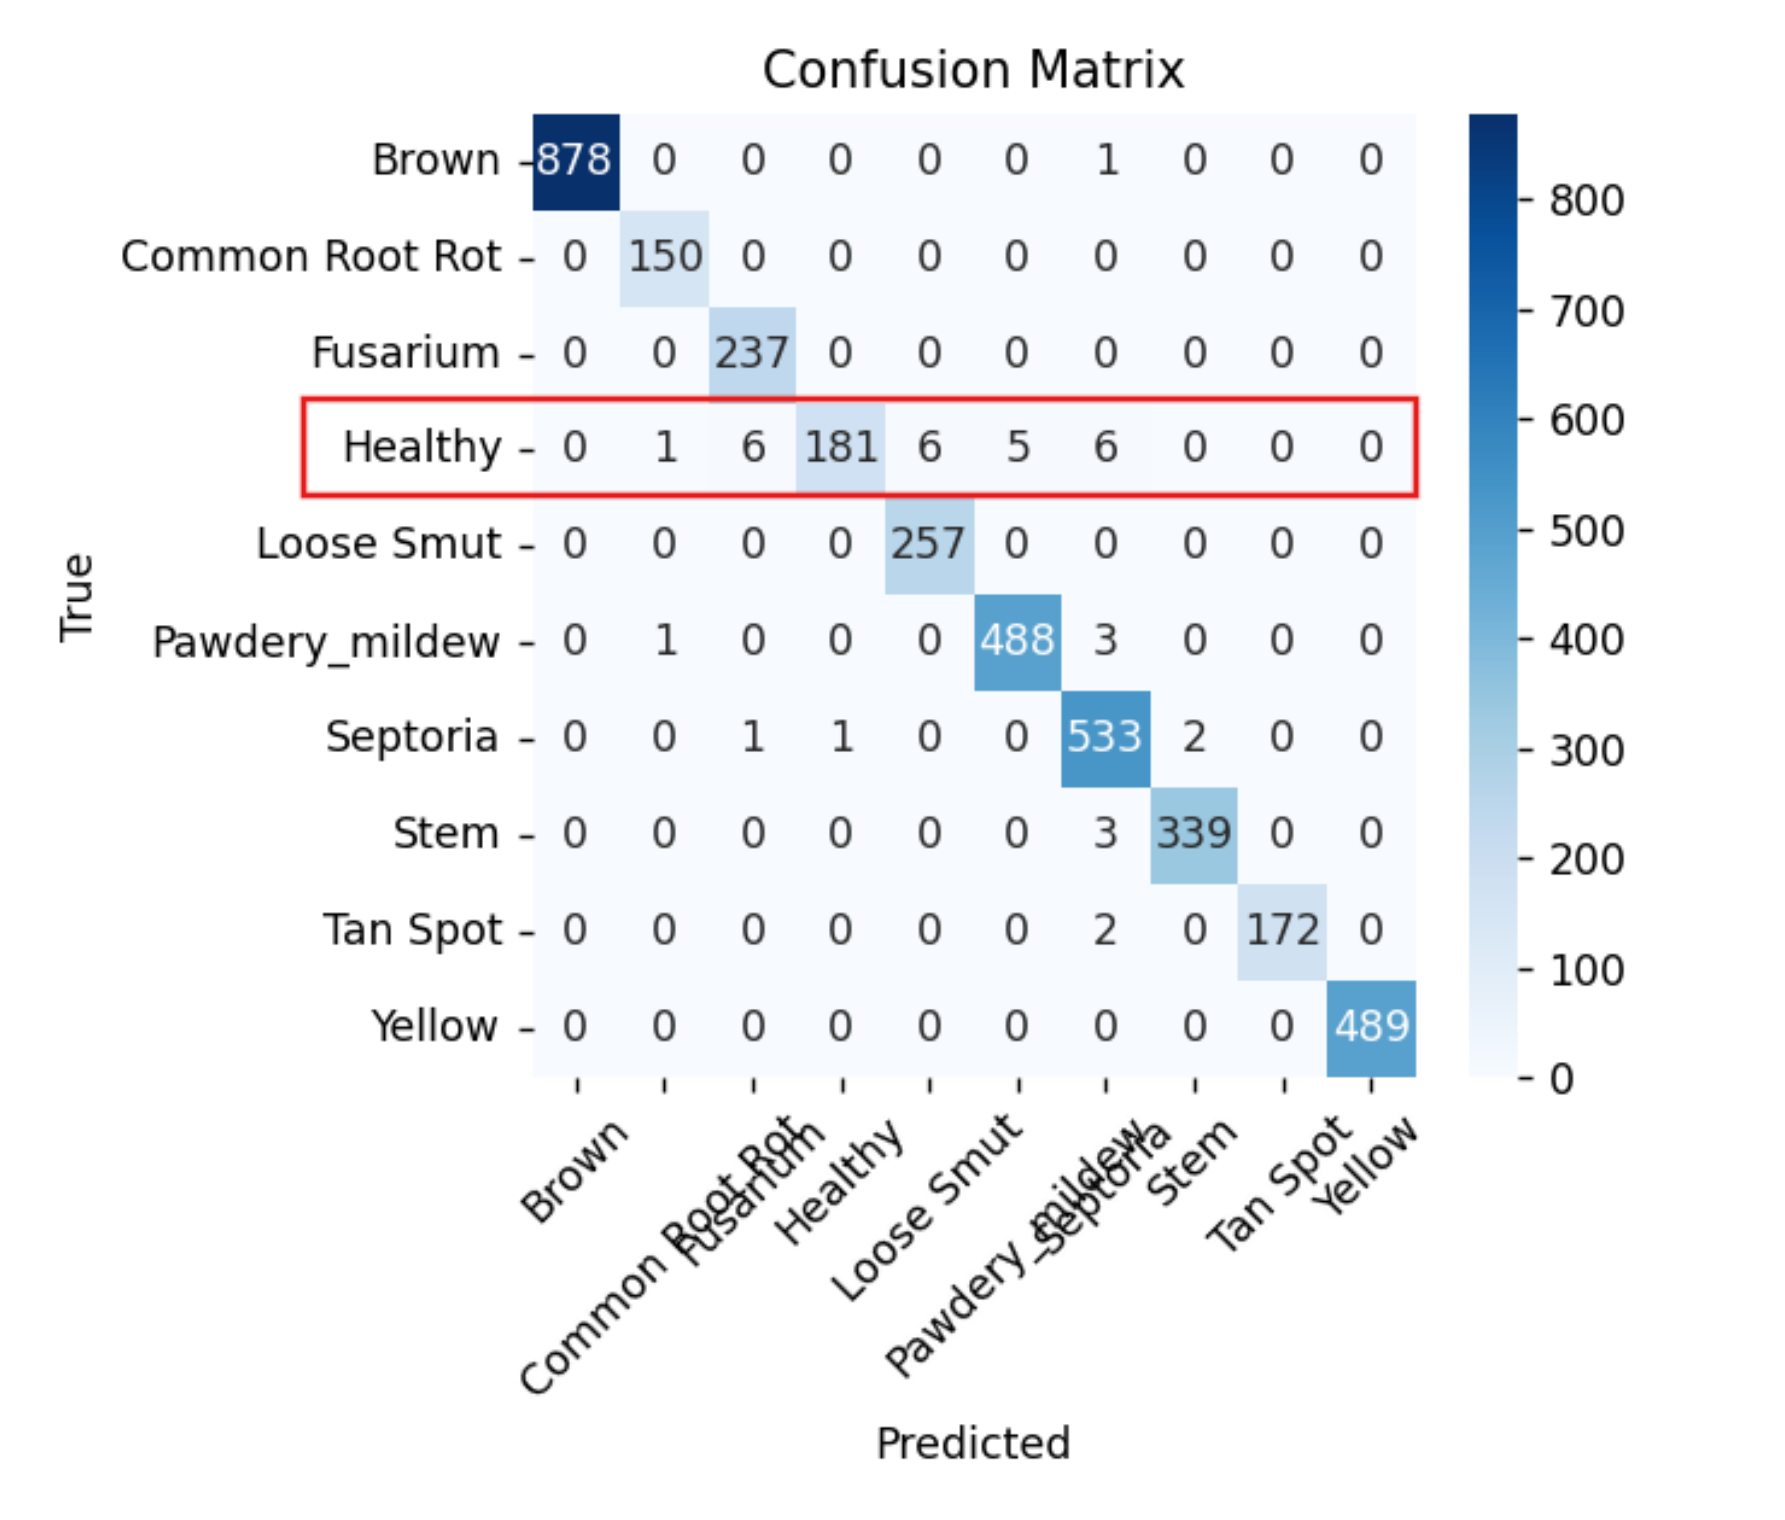
\includegraphics[width=0.8
\textwidth]{chapters/chapter56/images/ConfusionMatricsSingleModel.png}
\caption{Confusion Matrix of Model 2 for Multiclass Classification (10 Classes: Healthy + 9 Diseases)}
\label{fig:confusion_matrics_single_model}
\end{figure}


\section{Comparison with the State of the Art}

To assess the effectiveness of our proposed method, we conducted a comparative evaluation against two recent state-of-the-art studies. All approaches, including ours, were re-implemented under the same development environment and evaluated on our custom dataset, due to the unavailability of the original datasets used in the respective studies. This ensures a fair and consistent comparison.

The selection of the reference papers was guided by multiple criteria: the clarity and reproducibility of their reported hyperparameters, the availability of sufficient implementation details.

A summary of the re-implemented methods is presented in Table~\ref{tab:sota_studies}, which outlines the core components, configurations, and characteristics of each approach. The quantitative results of this comparison, including the performance of our proposed hierarchical approach, are reported in Table~\ref{tab:comparison_state_of_art}.

\begin{table}[H]
\centering
\renewcommand{\arraystretch}{1.4}
\setlength{\tabcolsep}{6pt}
\caption{Description of Re-implemented State-of-the-Art Approaches}
\label{tab:sota_studies}
\begin{tabular}{|p{2.5cm}|p{5cm}|p{5.5cm}|}
\hline
\textbf{Paper} & \textbf{Used Approach} & \textbf{Key Parameters and Hyperparameters} \\
\hline

% \textit{\parencite{goyal2021leaf}} & 
% Custom 24-layer deep CNN composed of 21 convolutional layers and 3 dense layers. The network uses ReLU/LeakyReLU activations, dropout regularization for overfitting control, and extensive data augmentation. It is trained with the Adam optimizer. & 
% \textbf{Model Parameters:}
% \begin{itemize}[leftmargin=*,noitemsep]
%     \item Input size: 224×224 RGB
% \end{itemize}
% \textbf{Training Hyperparameters:}
% \begin{itemize}[leftmargin=*,noitemsep]
%     \item Batch size: 32
%     \item Epochs: 1000 (early stopping applied)
%     \item Dropout: 0.25 (convolutional layers), 0.5 (dense layers)
%     \item Optimizer: Adam (default learning rate)
%     \item Augmentation: rotation (±20°), shift (20\%), horizontal/vertical flips
% \end{itemize} \\
% \hline

\textit{\parencite{fang2023lightweight}} & 
Modified Inception-ResNet architecture enhanced with Channel and Spatial Attention Modules (CBAM) and Efficient Channel Attention (ECA). Combines multiscale feature extraction with lightweight design. & 
\textbf{Model Parameters:}
\begin{itemize}[leftmargin=*,noitemsep]
    \item Input size: 224×224×3
    \item 4.24 million trainable parameters
\end{itemize}
\textbf{Training Hyperparameters:}
\begin{itemize}[leftmargin=*,noitemsep]
    \item Batch size: 64
    \item Epochs: 70
    \item Learning rate: 0.001 (StepLR decay: $\gamma=0.01$, step size=25)
    \item Weight decay: 0.001 (L2 regularization)
    \item Optimizer: Adam
\end{itemize} \\
\hline

\textit{\parencite{jouini2024wheat}} & 
Hybrid transfer learning pipeline combining frozen EfficientNetB0 for initial feature extraction with a shallow 3-layer custom CNN (filters: 32, 64, 128). & 
\textbf{Model Parameters:}
\begin{itemize}[leftmargin=*,noitemsep]
    \item Input size: 256×256 RGB
    \item 6 million trainable parameters
\end{itemize}
\textbf{Training Hyperparameters:}
\begin{itemize}[leftmargin=*,noitemsep]
    \item Batch size: 30
    \item Epochs: 100 (early stopping, patience=3)
    \item Optimizer: Adamax
    \item Dropout: 0.5
    \item Learning rate: 0.001 (adaptive reduction)
    \item Loss: Categorical cross-entropy
    \item Augmentation: rotation (±20°), shift (±20\%), zoom (0.8–1.2×)
\end{itemize} \\
\hline

\end{tabular}
\end{table}



\begin{table}[H]
\centering
\renewcommand{\arraystretch}{1.3}
\setlength{\tabcolsep}{6pt}
\caption{Comparative results between our approach and two state-of-the-art methods}
\begin{tabular}{|p{3cm}|p{2cm}|p{2cm}|p{2cm}|p{2cm}|p{2.5cm}|}
\hline
\textbf{Paper} & \textbf{Accuracy (\%)} & \textbf{Precision (\%)} & \textbf{Recall (\%)} & \textbf{F1-score (\%)} & \textbf{Avg Inference Time (ms)} \\
\hline
\parencite{fang2023lightweight}  & 85.00 & 83.00 & 82.00 & 82.00 & 9.705 \\
\hline
\parencite{jouini2024wheat}  & 94.41 & 94.59 & 94.41 &  94.40 & \textbf{5.91}\\
\hline
 Our Hierarchical approach & \textbf{99.48} & \textbf{99.38} & \textbf{99.18} & \textbf{99.31} & 8.0475 \\
\hline
\end{tabular}
\label{tab:comparison_state_of_art}
\end{table}



As shown in Table \ref{tab:comparison_state_of_art}, our hierarchical approach achieves superior results across all key metrics, with the highest accuracy (99.48\%), precision (99.38\%), recall (99.18\%), and F1-score (99.31\%), significantly outperforming the compared state-of-the-art methods.

In terms of inference time, our model remains highly efficient at 8.05 ms, with only a marginal increase compared to \textcite{jouini2024wheat} (5.91 ms). This minimal difference is outweighed by the substantial gains in predictive performance. The added complexity introduced by the two-stage structure is minimal, yet it brings a notable advantage in classification quality. This makes our approach not only highly accurate but also practical for real-time deployment, especially in precision agriculture scenarios where both speed and reliability are critical.





\section{Evaluating Insect Pest Detection Model}
\label{sec:Pesttest}
To evaluate the performance of our insect pest detection model, we created and annotated a dedicated dataset. The annotation process was conducted in two phases:

\begin{itemize}
    \item \textbf{First Phase – Standard Bounding Boxes (YOLOv8)}: In the initial phase, we used regular (horizontal) bounding boxes aligned with image axes. Each insect instance was enclosed in a rectangular box defined by four parameters: $(x, y, w, h)$, representing the top-left coordinates and width/height of the box.
    
    \item \textbf{Second Phase – Oriented Bounding Boxes (YOLOv8-OBB)}: In the second phase, we used oriented bounding boxes (OBBs), which allow for rotation. These are defined by five parameters: $(x, y, w, h, \theta)$, where $\theta$ indicates the angle of rotation. This approach enables more precise localization, especially for insects captured at various orientations.
\end{itemize}

We trained and evaluated two versions of the YOLOv8 model on the same dataset using two different annotation styles: one with standard bounding boxes and the other with oriented bounding boxes. The evaluation results are summarized in Table~\ref{tab:yolo_comparison}, which clearly shows that the YOLOv8-OBB variant outperforms the standard version across all key metrics.
\begin{table}[H]
\centering
\renewcommand{\arraystretch}{1.5}
\setlength{\tabcolsep}{8pt}
\caption{Comparison Between YOLOv8 with Oriented Bounding Boxes (OBB) and Standard YOLOv8}
\begin{tabular}{|c|c|c|p{6cm}|}
\hline
\textbf{Metric} & \textbf{YOLOv8-OBB} & \textbf{YOLOv8 (Standard)} & \textbf{Interpretation} \\
\hline
Precision (P) & 0.945 & 0.809 & OBB predicts fewer false positives. \\
\hline
Recall (R) & 0.862 & 0.564 & OBB detects more true positives. \\
\hline
mAP@0.5 & 0.924 & 0.708 & OBB shows much higher detection quality at 0.5 IoU. \\
\hline
mAP@0.5:0.95 & 0.683 & 0.474 & OBB performs better across stricter IoU thresholds. \\
\hline
\end{tabular}
\label{tab:yolo_comparison}
\end{table}

The comparison in Table~\ref{tab:yolo_comparison} clearly demonstrates that the YOLOv8 model using Oriented Bounding Boxes (YOLOv8-OBB) provides a noticeable improvement over the standard version. The OBB-based model achieves better precision and recall, which indicates a stronger ability to correctly identify insect pests while reducing false detections.

Moreover, the higher mAP scores across both standard and stricter IoU thresholds suggest that the OBB model maintains more accurate detections in varied conditions. This is especially important in real-world scenarios where pests can appear in diverse orientations and poses.

Figure~\ref{fig:ConfusionMatricsPests} shows fewer misclassifications in the OBB-based model, reflecting improved class-wise performance. Additionally, Figure~\ref{fig:YoloObbResualts} highlights how oriented boxes more effectively adapt to the shape and rotation of insect targets, supporting the practical benefits of using OBB annotations in the field.

\begin{figure}[H] % 'H' needs \usepackage{float}
    \centering
    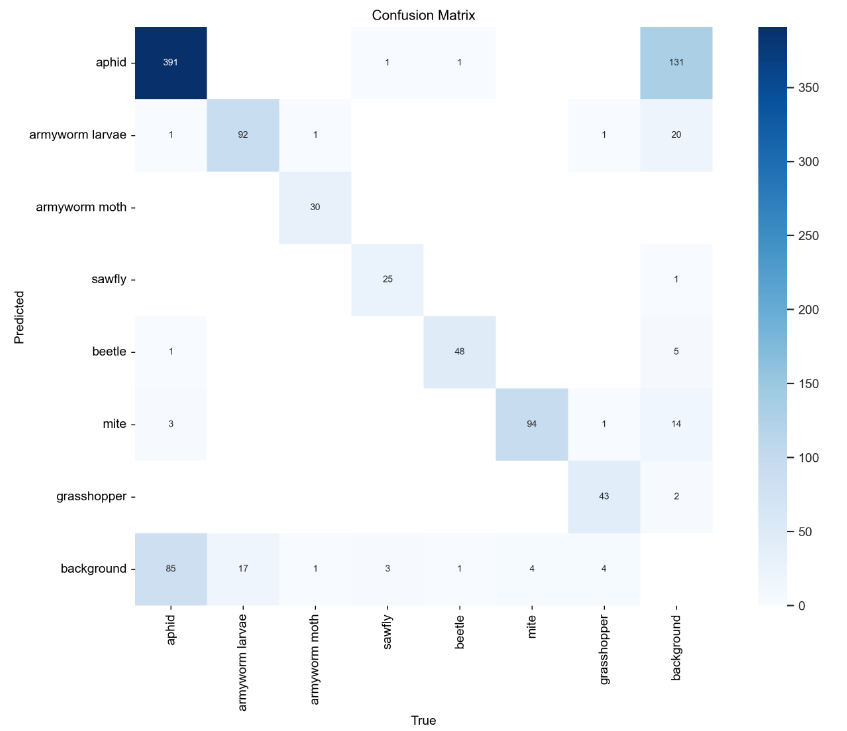
\includegraphics[width=0.9\textwidth]{chapters/chapter56/images/ConfusionMatricsPests.png}
    \caption{Confusion matrics of Insect detection model.}
    \label{fig:ConfusionMatricsPests}
\end{figure}

\begin{figure}[H] % 'H' needs \usepackage{float}
    \centering
    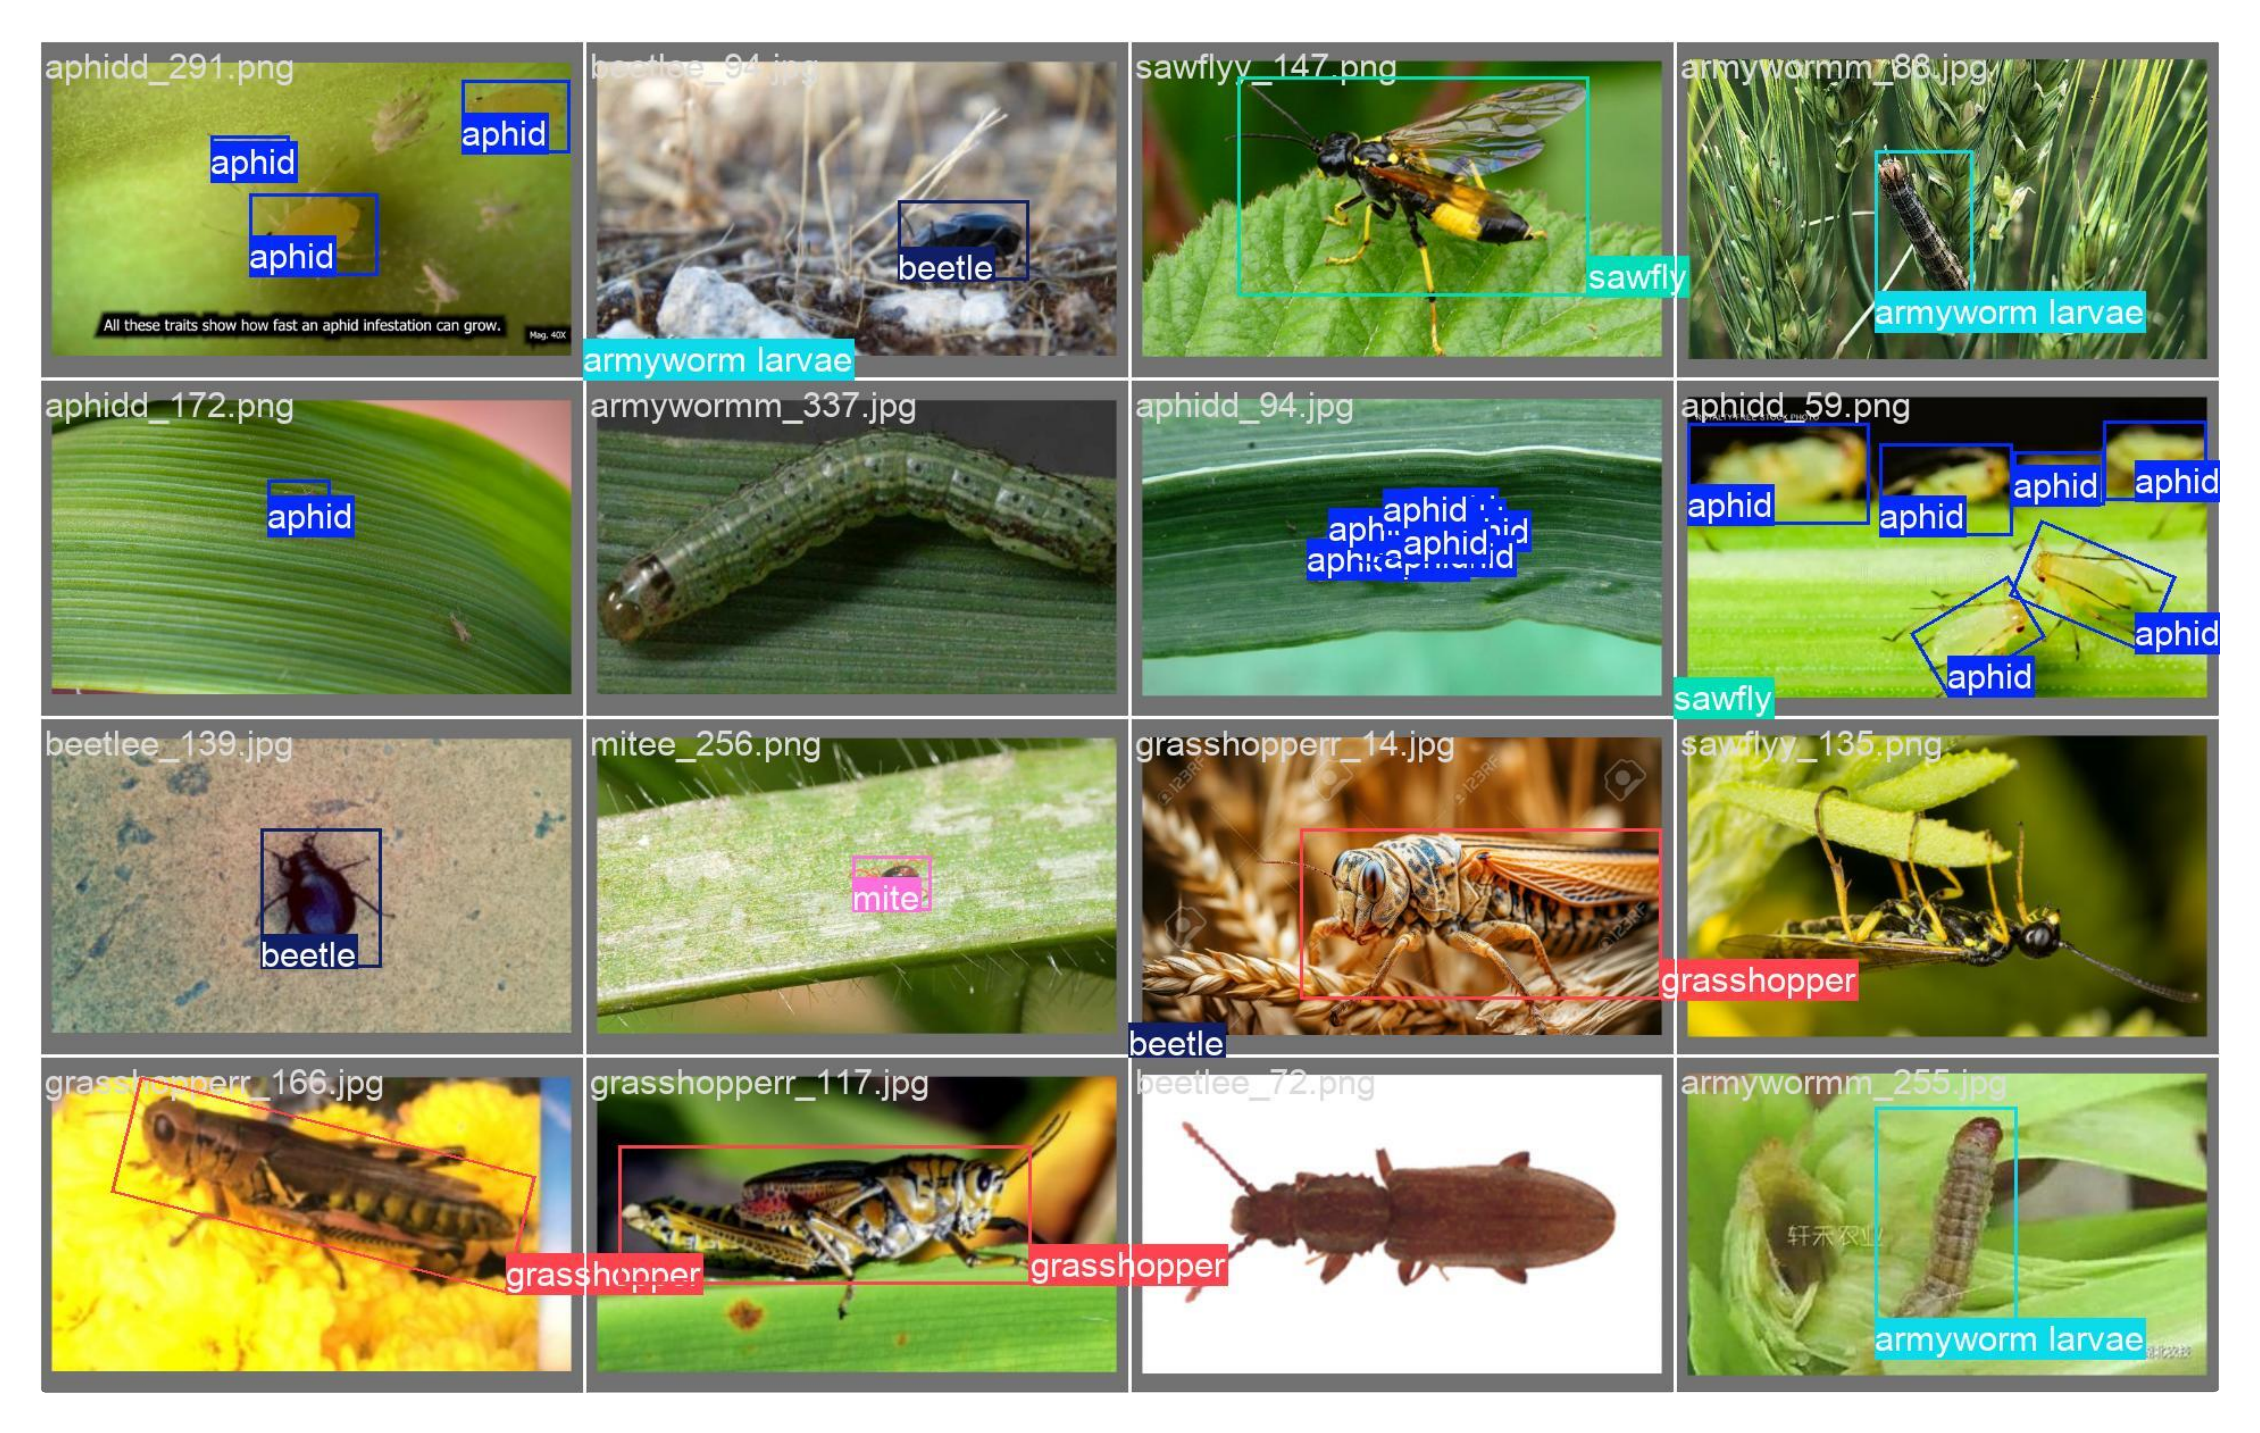
\includegraphics[width=0.9\textwidth]{chapters/chapter56/images/YoloObbResualts.png}
    \caption{Insect detection model results.}
    \label{fig:YoloObbResualts}
\end{figure}


\section{Conclusion}



This chapter demonstrated the successful implementation of all core components of the proposed system. The results obtained from extensive experiments confirmed the reliability and performance of the wheat disease classification and pest detection models. The deployment into a responsive web platform, along with the integration of an AI assistant, further emphasizes the practical usability of the solution in real agricultural settings. Comparisons with existing approaches also highlighted the competitive edge of our system in terms of accuracy, generalization, and ease of use, fulfilling the objectives defined in the early stages of this work.










